% Compile with LuaLaTeX
%
\documentclass[%handout
]{beamer}

\usepackage{geometry}
\geometry{paperwidth=160mm, paperheight=115mm, left = 5mm}

\usepackage{polyglossia}
\setmainlanguage[]{french}

%% Table
\usepackage{longtable}
\usepackage{booktabs}
\usepackage[skip =0pt, position=auto]{caption}

\usepackage{graphicx}

\usepackage{natbib}
\bibliographystyle{apalike}
\renewcommand{\bibsection}{\subsubsection*{\bibname } }

\usepackage{fontawesome}

\usetheme{metropolis}           % Use metropolis theme

\metroset{block=fill}

\setbeamertemplate{title page}{
  \begin{minipage}[b][\paperheight]{\textwidth}
    \ifx\inserttitlegraphic\@empty\else\usebeamertemplate*{title graphic}\fi
    \vfill%
    \ifx\inserttitle\@empty\else\usebeamertemplate*{title}\fi
    \ifx\insertsubtitle\@empty\else\usebeamertemplate*{subtitle}\fi
    \usebeamertemplate*{title separator}
    \begin{minipage}[t]{.5\textwidth}
    \ifx\beamer@shortauthor\@empty\else\usebeamertemplate*{author}\fi
    \ifx\insertdate\@empty\else\usebeamertemplate*{date}\fi
    \ifx\insertinstitute\@empty\else\usebeamertemplate*{institute}\fi
    \end{minipage}
    \begin{minipage}[t]{.5\textwidth}
    \vspace*{3em}
    {\footnotesize Dr Martin Marzloff, Dr Aurélien Boyé,\par Dr Olivier Gauthier, Dr Jacques Grall%
    \par}
    \end{minipage}
    \vspace{\baselineskip}\\
    
\includegraphics[scale=0.9]{figs/logo_memoire.png}
    \vspace*{1mm}
  \end{minipage}
}

\usepackage{appendixnumberbeamer}


\title{Caractériser la contribution des facteurs environnementaux et des interactions biotiques à la variabilité des assemblages benthiques}
\date{16 juin 2020}
\author{Clément VIOLET}
\institute{Université de Rennes 1 \par Laboratoire d'Ecologie Benthique Cotière}

%%%%%%%%%%%%%%%%%%%%%%%%%%%%%%%%%%%%%%%%%%%
%                                         %
%   Début diapo                           %
%                                         %
%%%%%%%%%%%%%%%%%%%%%%%%%%%%%%%%%%%%%%%%%%%
\begin{document}

  \maketitle
  
  \section{Problématique \& méthodologie}

  \begin{frame}{Niche environnementale}
	Capacité de persistance d'une espèce $\rightarrow$ niche à n-dimensions~\citep{Hutchinson_1957}\\\vspace{2\baselineskip}
	\pause
	\begin{figure}[t]
		\begin{center}
			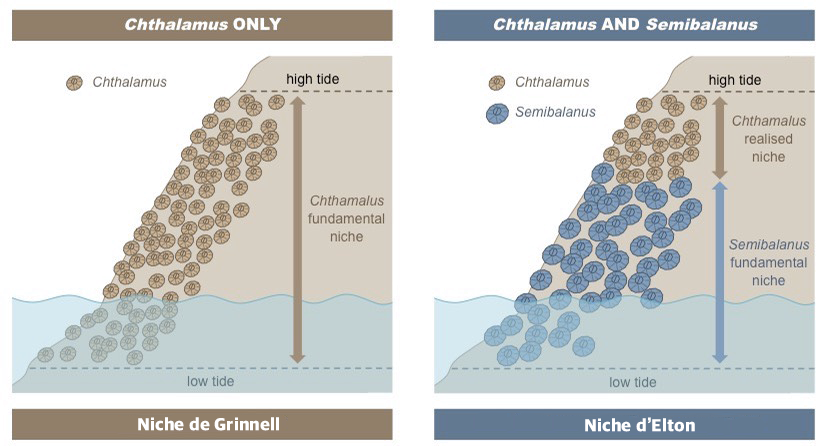
\includegraphics[scale = 0.43]{figs/barnacle1_med.png}
		\end{center}
	\end{figure}
	\end{frame}
	
	\begin{frame}{Etudier une niche environnementale}
	\begin{figure}[t]
		\begin{center}
			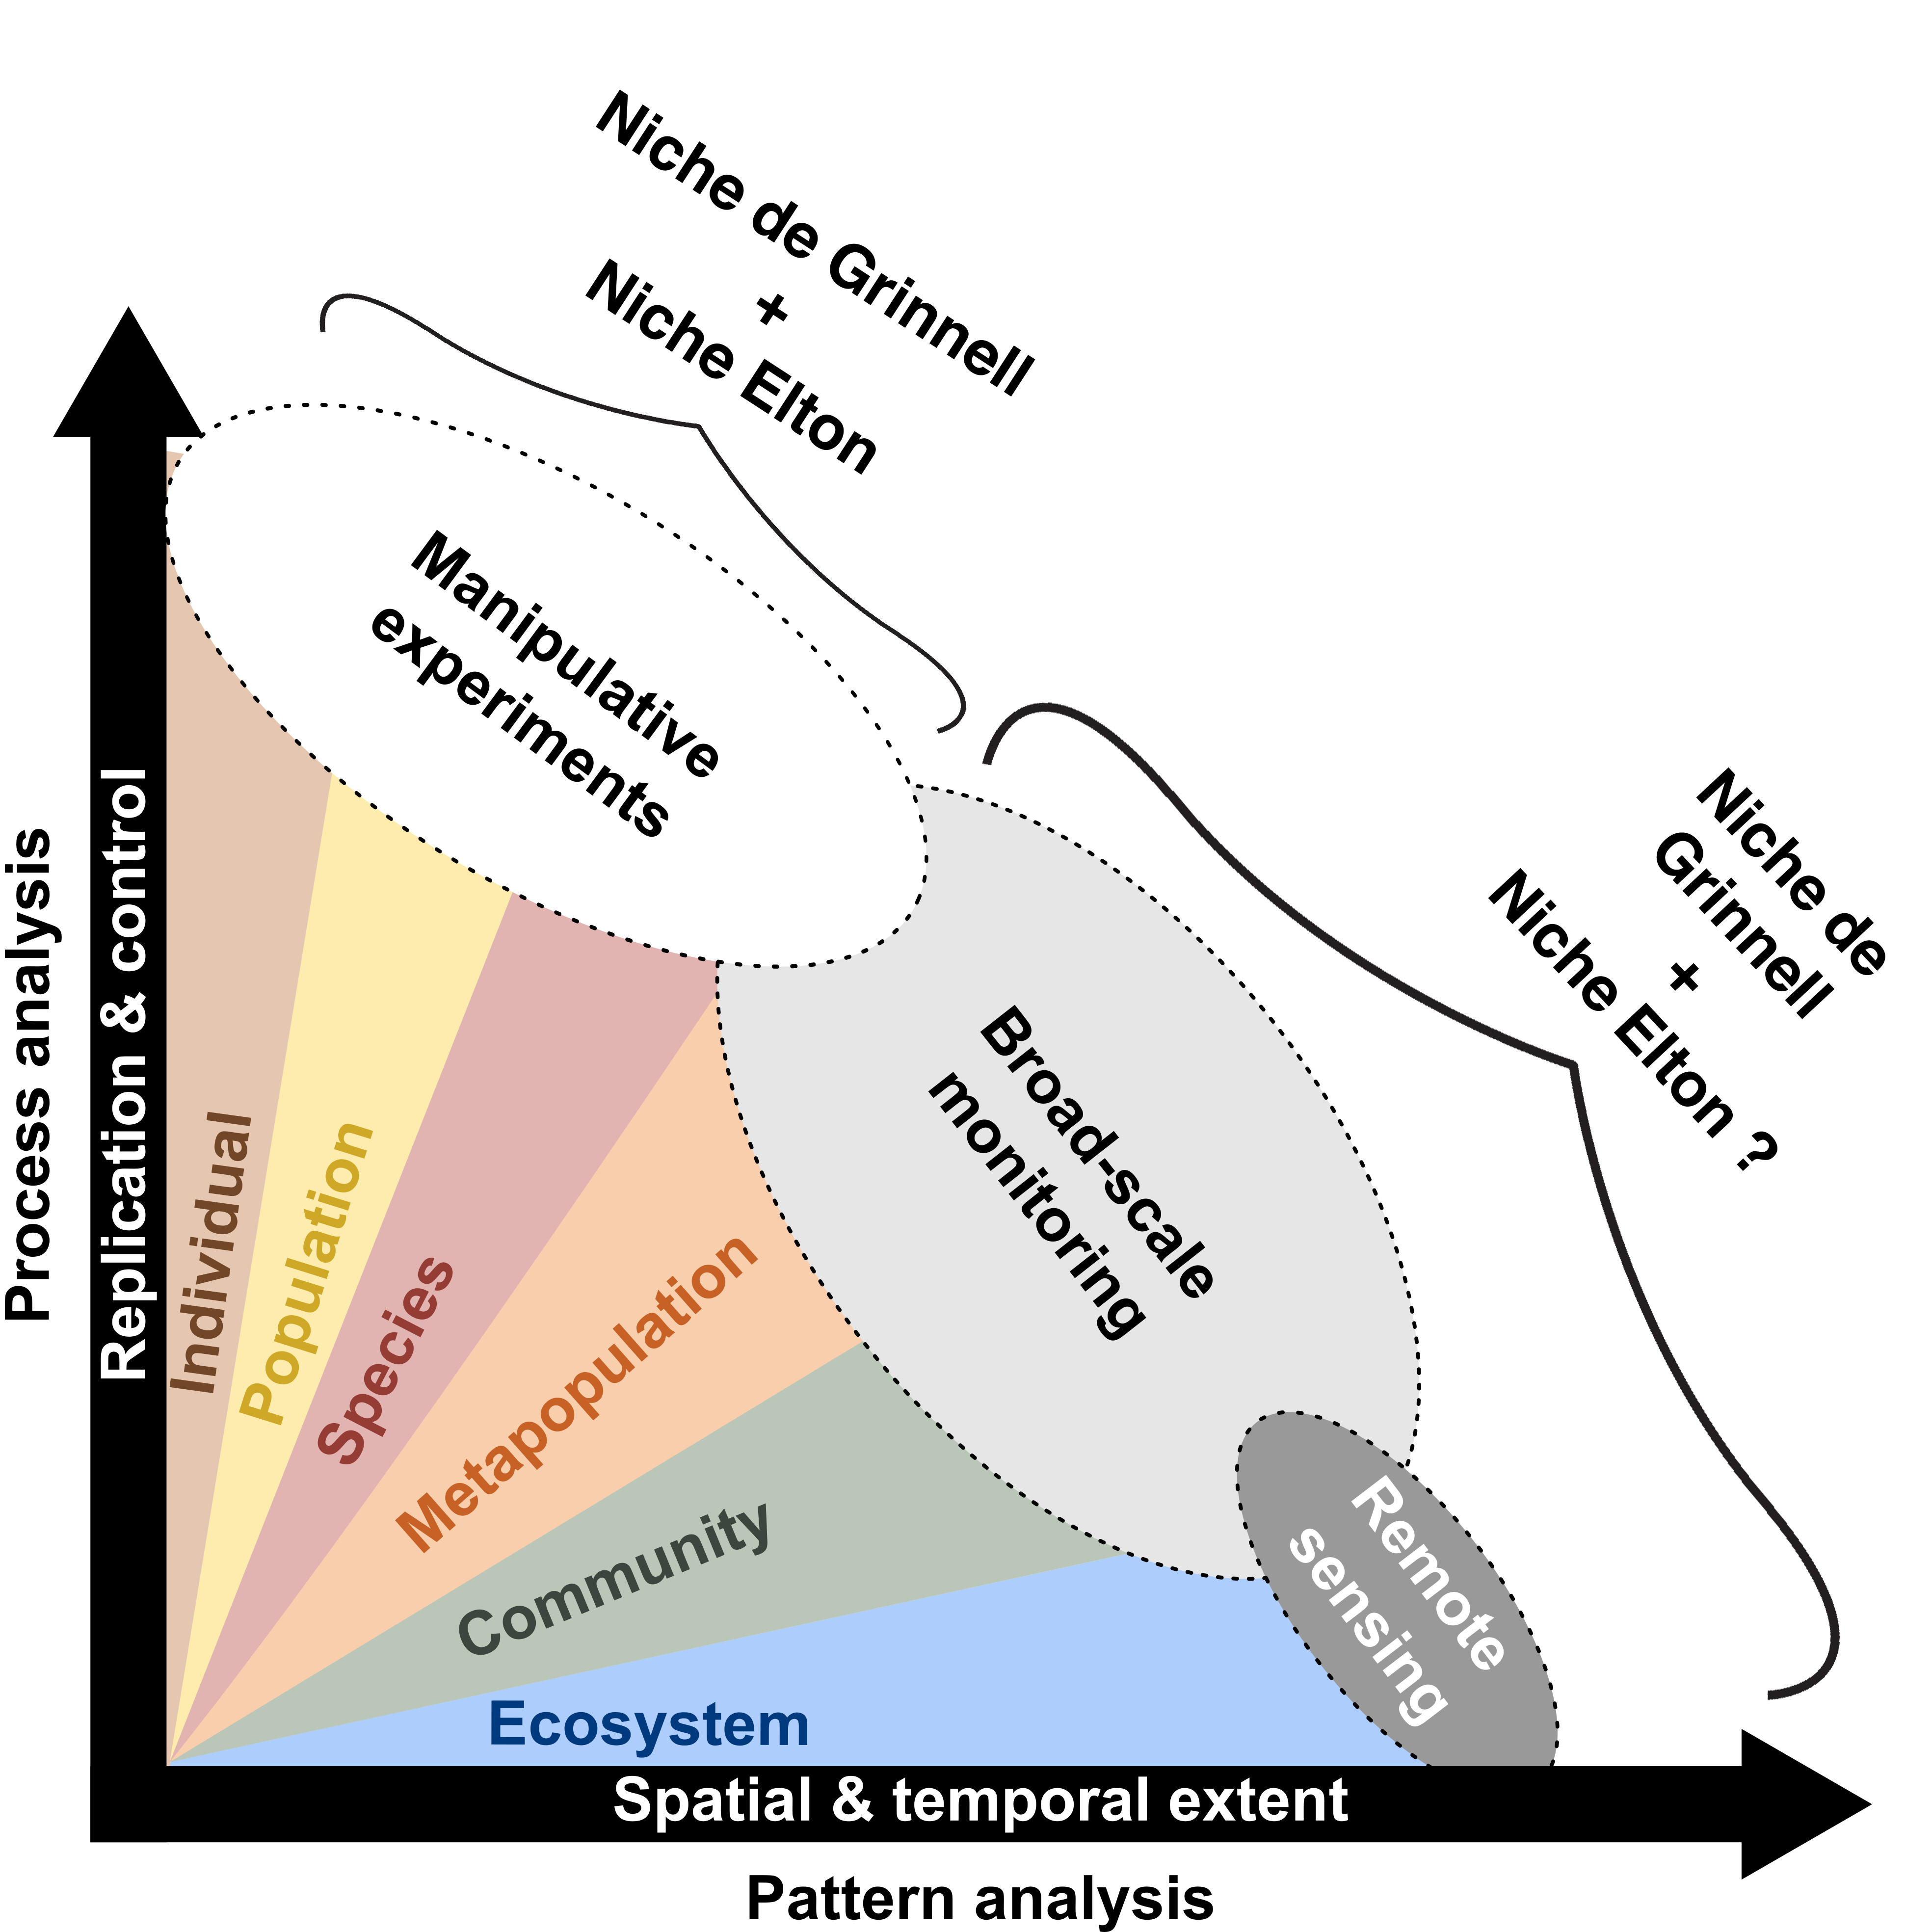
\includegraphics[scale = 0.07]{figs/Fig_scale_monitoring_3.png}
		\end{center}
	\end{figure}
	\end{frame}
	
	\begin{frame}{Modèles de distribution d'espèces}
		\emph{Species Distribution Models} (\emph{SDM})\vspace{\baselineskip}\\
	\begin{figure}[t]
		\begin{center}
			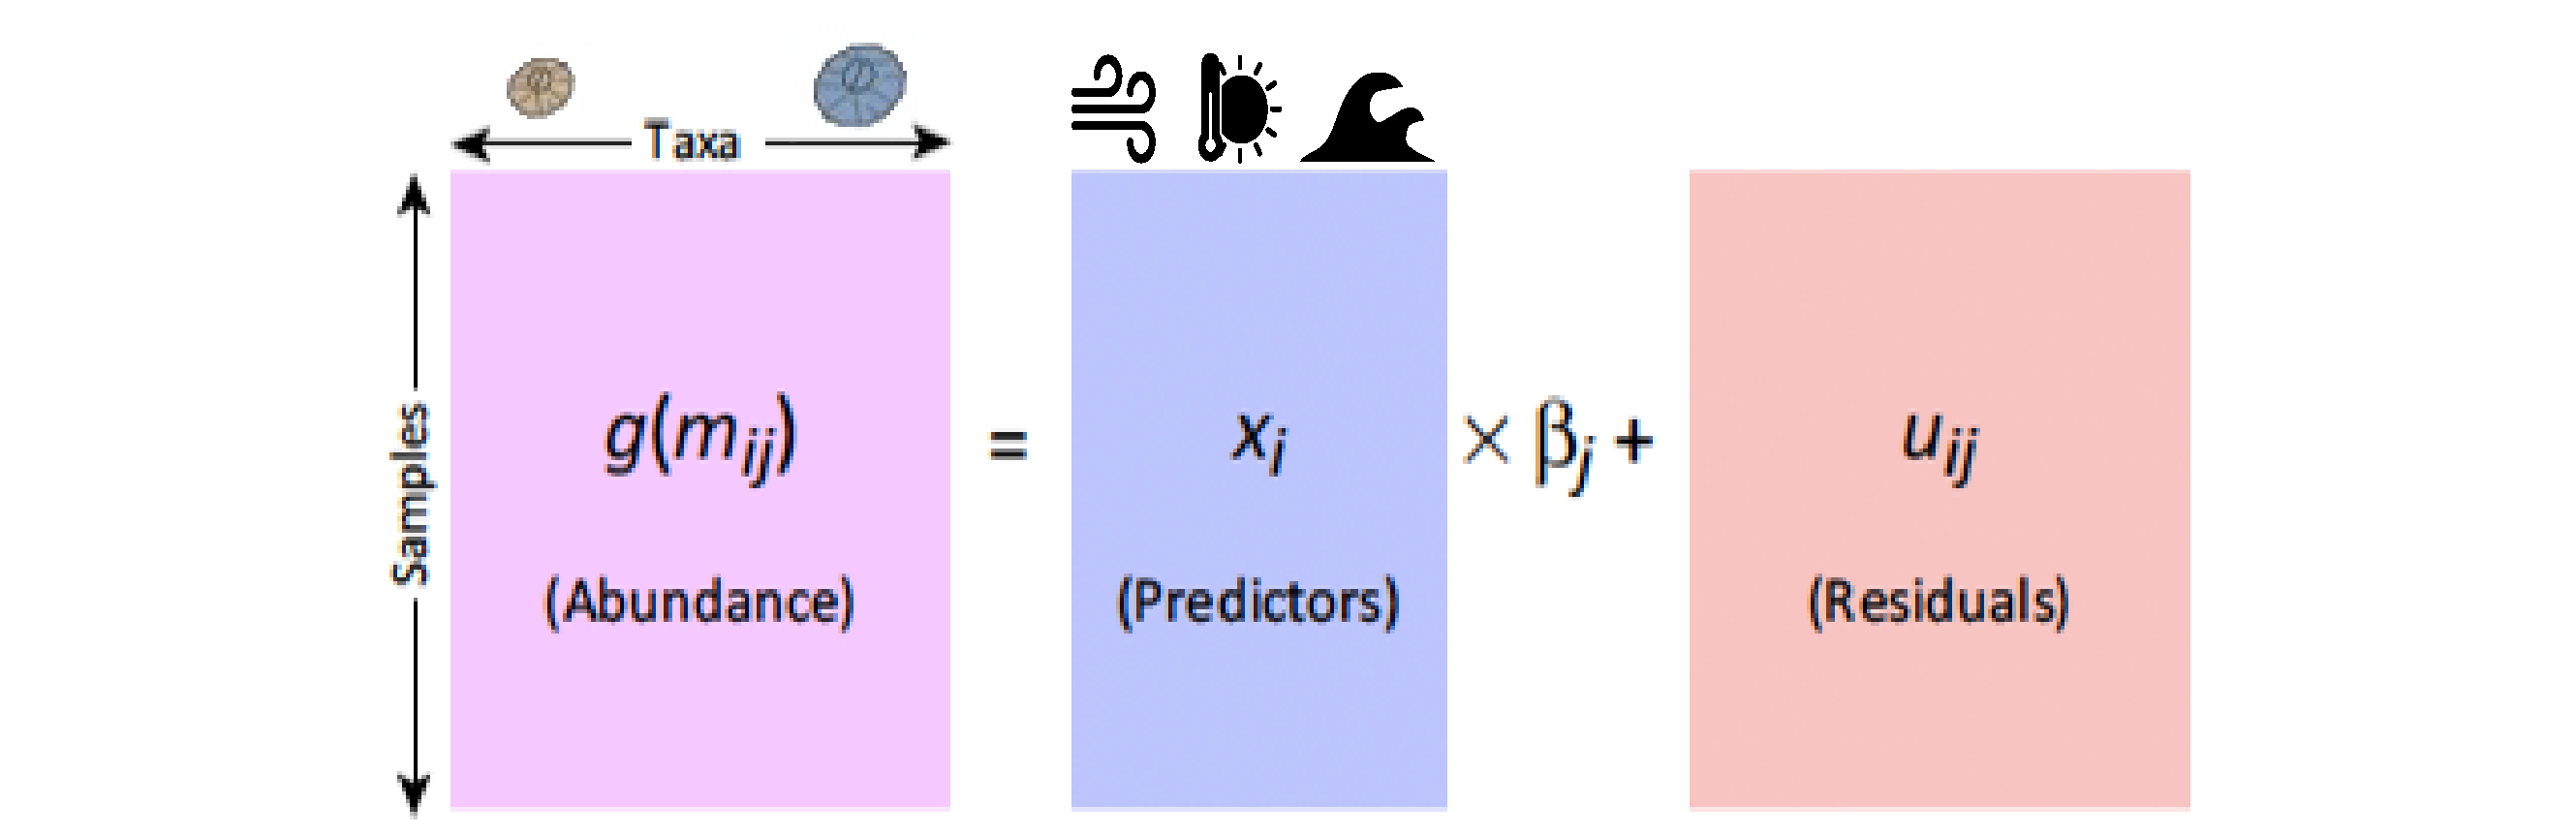
\includegraphics[scale = 0.1]{figs/glm.png}
		\end{center}
	\end{figure}\pause
		\emph{Joint Species Distribution Models} (\emph{JSDM})
		\begin{figure}[t]
		\begin{center}
			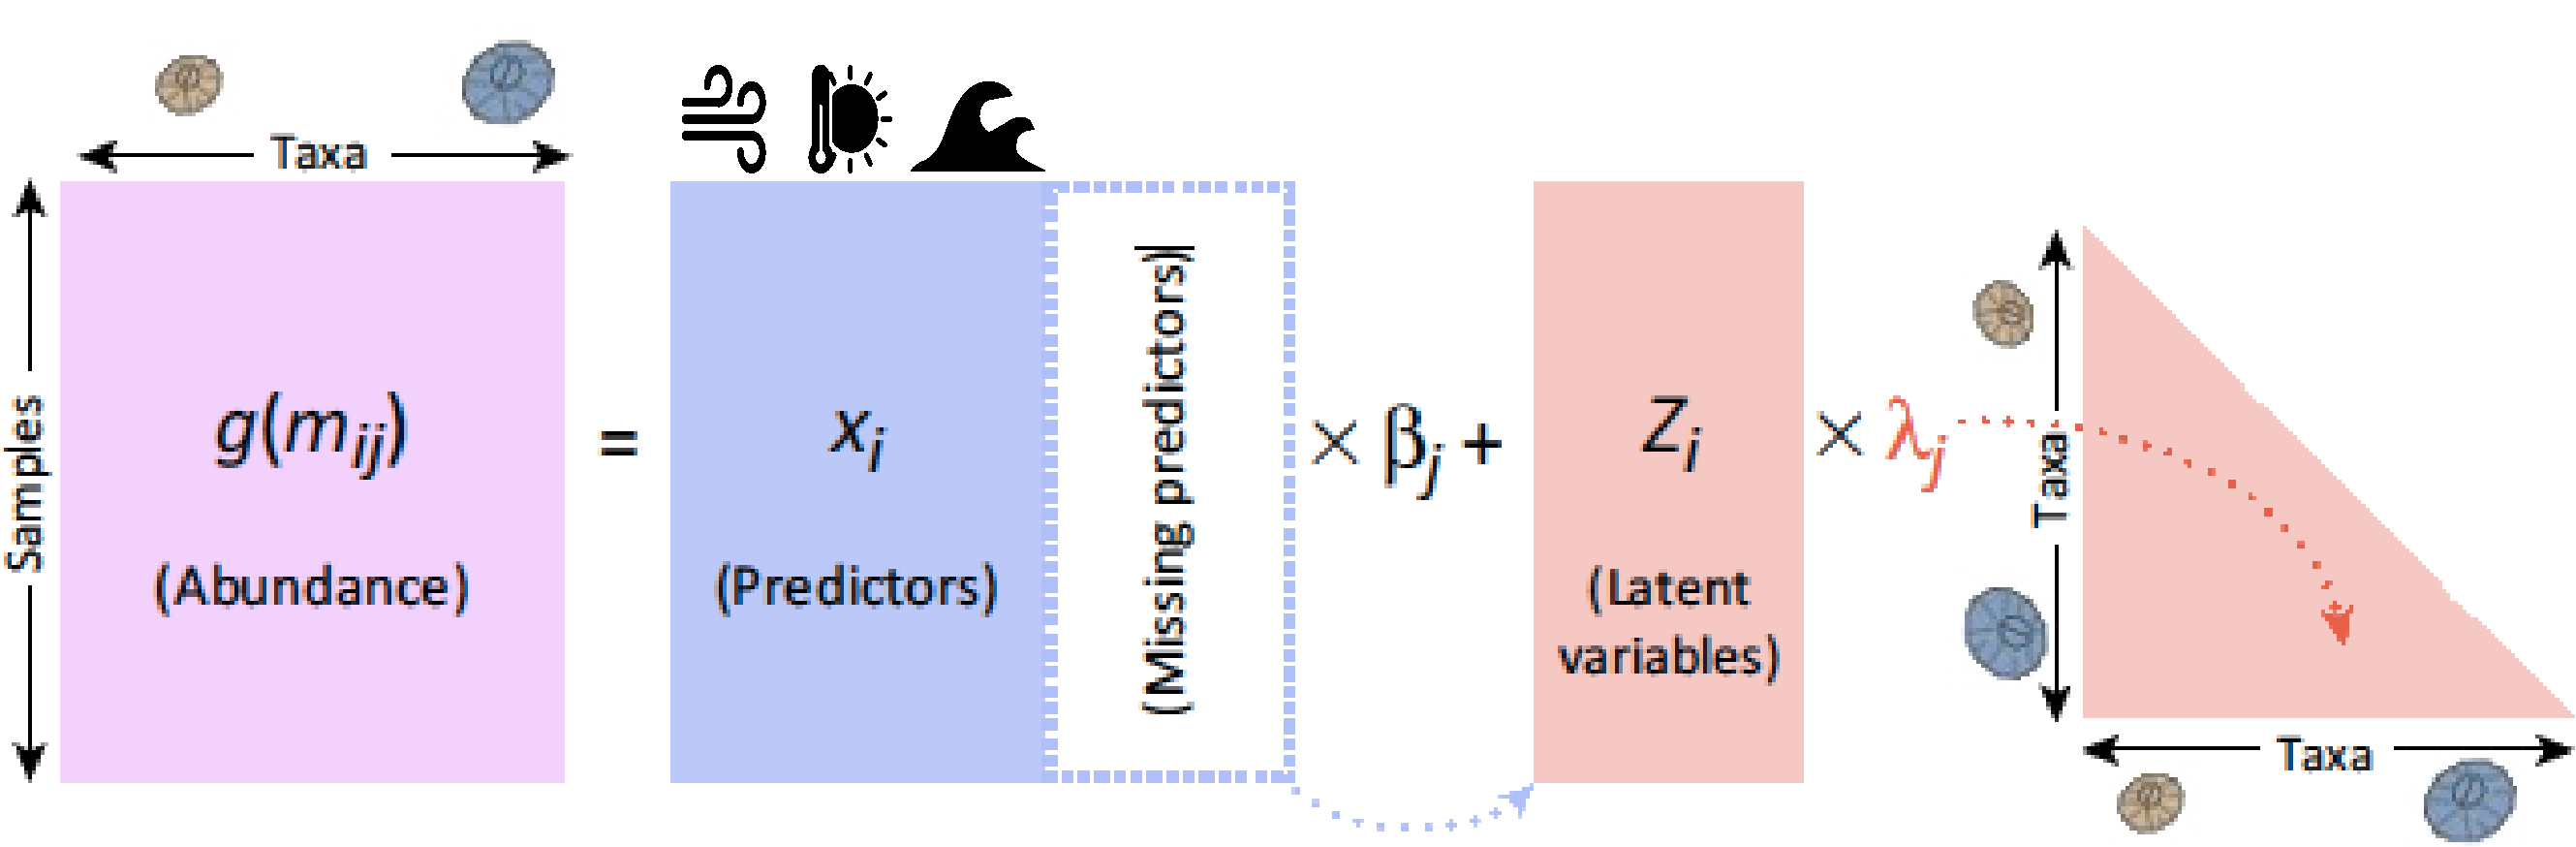
\includegraphics[scale = 0.1]{figs/lvm3.png}
		\end{center}
	\end{figure}
	\end{frame}
	
	\begin{frame}{Méthodologie}
	3 \emph{JSDM} comparés (5 variants au total) :
	\begin{scriptsize}
		\begin{longtable}[]{lllll}
		\toprule
		\begin{minipage}[b]{0.11\columnwidth}\raggedright
		Nom du modèle\strut
		\end{minipage} & \begin{minipage}[b]{0.09\columnwidth}\raggedright
		Framework\strut
		\end{minipage} & \begin{minipage}[b]{0.19\columnwidth}\raggedright
		Distribution statistique\strut
		\end{minipage} & \begin{minipage}[b]{0.24\columnwidth}\raggedright
		Nombre de facteurs aléatoires\strut
		\end{minipage} & \begin{minipage}[b]{0.22\columnwidth}\raggedright
		Nombre de variables latentes\strut
		\end{minipage}\tabularnewline
		\toprule
		\endfirsthead
		\toprule
		\begin{minipage}[b]{0.11\columnwidth}\raggedright
		Nom du modèle\strut
		\end{minipage} & \begin{minipage}[b]{0.09\columnwidth}\raggedright
		Framework\strut
		\end{minipage} & \begin{minipage}[b]{0.19\columnwidth}\raggedright
		Distribution statistique\strut
		\end{minipage} & \begin{minipage}[b]{0.24\columnwidth}\raggedright
		Nombre de facteurs aléatoires\strut
		\end{minipage} & \begin{minipage}[b]{0.22\columnwidth}\raggedright
		Nombre de variables latentes\strut
		\end{minipage}\tabularnewline
		\toprule
		\endhead
		\begin{minipage}[t]{0.11\columnwidth}\raggedright
		\emph{HMSC\_reg}\strut
		\end{minipage} & \begin{minipage}[t]{0.09\columnwidth}\raggedright
		\emph{HMSC}\strut
		\end{minipage} & \begin{minipage}[t]{0.19\columnwidth}\raggedright
		Poisson lognormal\strut
		\end{minipage} & \begin{minipage}[t]{0.24\columnwidth}\raggedright
		0\strut
		\end{minipage} & \begin{minipage}[t]{0.22\columnwidth}\raggedright
		\(0\)\strut
		\end{minipage}\tabularnewline
		\begin{minipage}[t]{0.11\columnwidth}\raggedright
		\emph{HMSC\_samp}\strut
		\end{minipage} & \begin{minipage}[t]{0.09\columnwidth}\raggedright
		\emph{HMSC}\strut
		\end{minipage} & \begin{minipage}[t]{0.19\columnwidth}\raggedright
		Poisson lognormal\strut
		\end{minipage} & \begin{minipage}[t]{0.24\columnwidth}\raggedright
		1\strut
		\end{minipage} & \begin{minipage}[t]{0.22\columnwidth}\raggedright
		\(n_l \in \mathbb{N}^*\)\strut
		\end{minipage}\tabularnewline
		\begin{minipage}[t]{0.11\columnwidth}\raggedright
		\emph{HMSC\_hier}\strut
		\end{minipage} & \begin{minipage}[t]{0.09\columnwidth}\raggedright
		\emph{HMSC}\strut
		\end{minipage} & \begin{minipage}[t]{0.19\columnwidth}\raggedright
		Poisson lognormal\strut
		\end{minipage} & \begin{minipage}[t]{0.24\columnwidth}\raggedright
		3\strut
		\end{minipage} & \begin{minipage}[t]{0.22\columnwidth}\raggedright
		\(n_l \in \mathbb{N}^*\)\strut
		\end{minipage}\tabularnewline\midrule%\pause
		\begin{minipage}[t]{0.11\columnwidth}\raggedright
		\emph{PLN}\strut
		\end{minipage} & \begin{minipage}[t]{0.09\columnwidth}\raggedright
		\emph{PLN}\strut
		\end{minipage} & \begin{minipage}[t]{0.19\columnwidth}\raggedright
		Poisson lognormal\strut
		\end{minipage} & \begin{minipage}[t]{0.24\columnwidth}\raggedright
		1\strut
		\end{minipage} & \begin{minipage}[t]{0.22\columnwidth}\raggedright
		\(n_l = 92\)\strut
		\end{minipage}\tabularnewline\midrule%\pause
		\begin{minipage}[t]{0.11\columnwidth}\raggedright
		\emph{GLLVM}\strut
		\end{minipage} & \begin{minipage}[t]{0.09\columnwidth}\raggedright
		\emph{GLLVM}\strut
		\end{minipage} & \begin{minipage}[t]{0.19\columnwidth}\raggedright
		Negative binomial\strut
		\end{minipage} & \begin{minipage}[t]{0.24\columnwidth}\raggedright
		0\strut
		\end{minipage} & \begin{minipage}[t]{0.22\columnwidth}\raggedright
		\(20\)\strut
		\end{minipage}\tabularnewline
		\bottomrule
		\end{longtable}
	\end{scriptsize}\vspace{\baselineskip}
	\begin{figure}[t]
		\begin{center}
			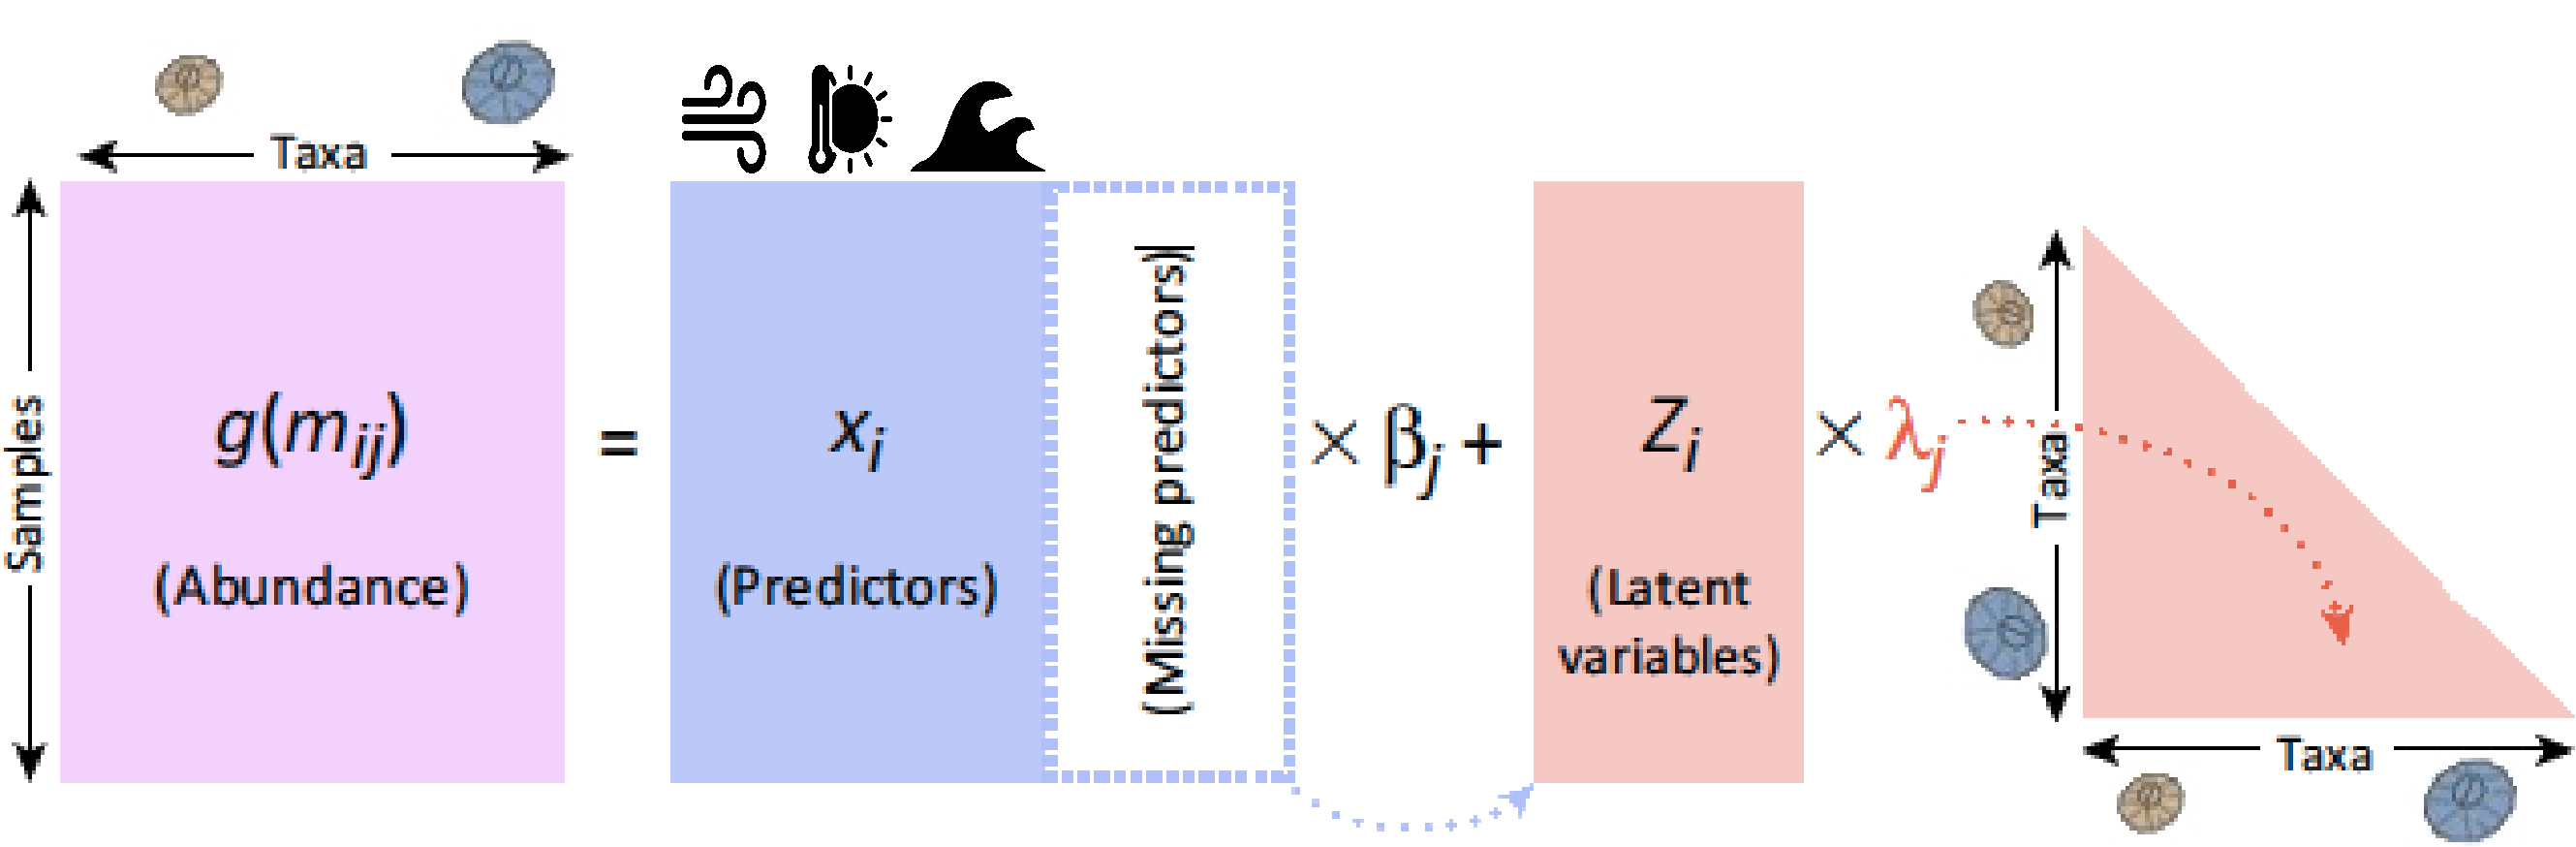
\includegraphics[scale = 0.14]{figs/lvm3.png}
		\end{center}
	\end{figure}
	\end{frame}
	
	\begin{frame}{Méthodologie}
		Réseau reconstruit par méthode \emph{EMtree}~\citep{Momal_2020}.\vspace{0.5\baselineskip}
		\begin{figure}[t]
		\begin{center}
			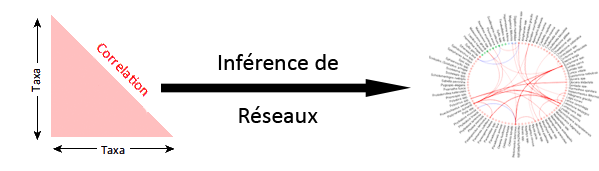
\includegraphics[scale =0.65]{figs/network_inf.png}
		\end{center}
		\end{figure}
	\end{frame}
	
	\begin{frame}{Cas d'étude}
	Données faunistiques issues du 
\includegraphics[scale=0.2]{figs/LogoREBENT.png} :~\citep{Boye_2019a}
	\begin{itemize}
		\item Macrofaune benthique ($> 1\text{mm}$) $\rightarrow$ polychètes (96 taxa)
		\item 8 ans de suivis + 23 sites (215 unités d'échantillonnages)
	\end{itemize}
	Données environnementales 7 variables : 
\includegraphics[scale=0.2]{figs/noun_Hot.png}, 
\includegraphics[scale=0.2]{figs/noun_Wind.png}, 
\includegraphics[scale=0.2]{figs/noun_Salt.png}, 
\includegraphics[scale=0.2]{figs/noun_wave.png}, 
\includegraphics[scale=0.2]{figs/noun_sand.png}
		\begin{figure}[t]
		\begin{center}
			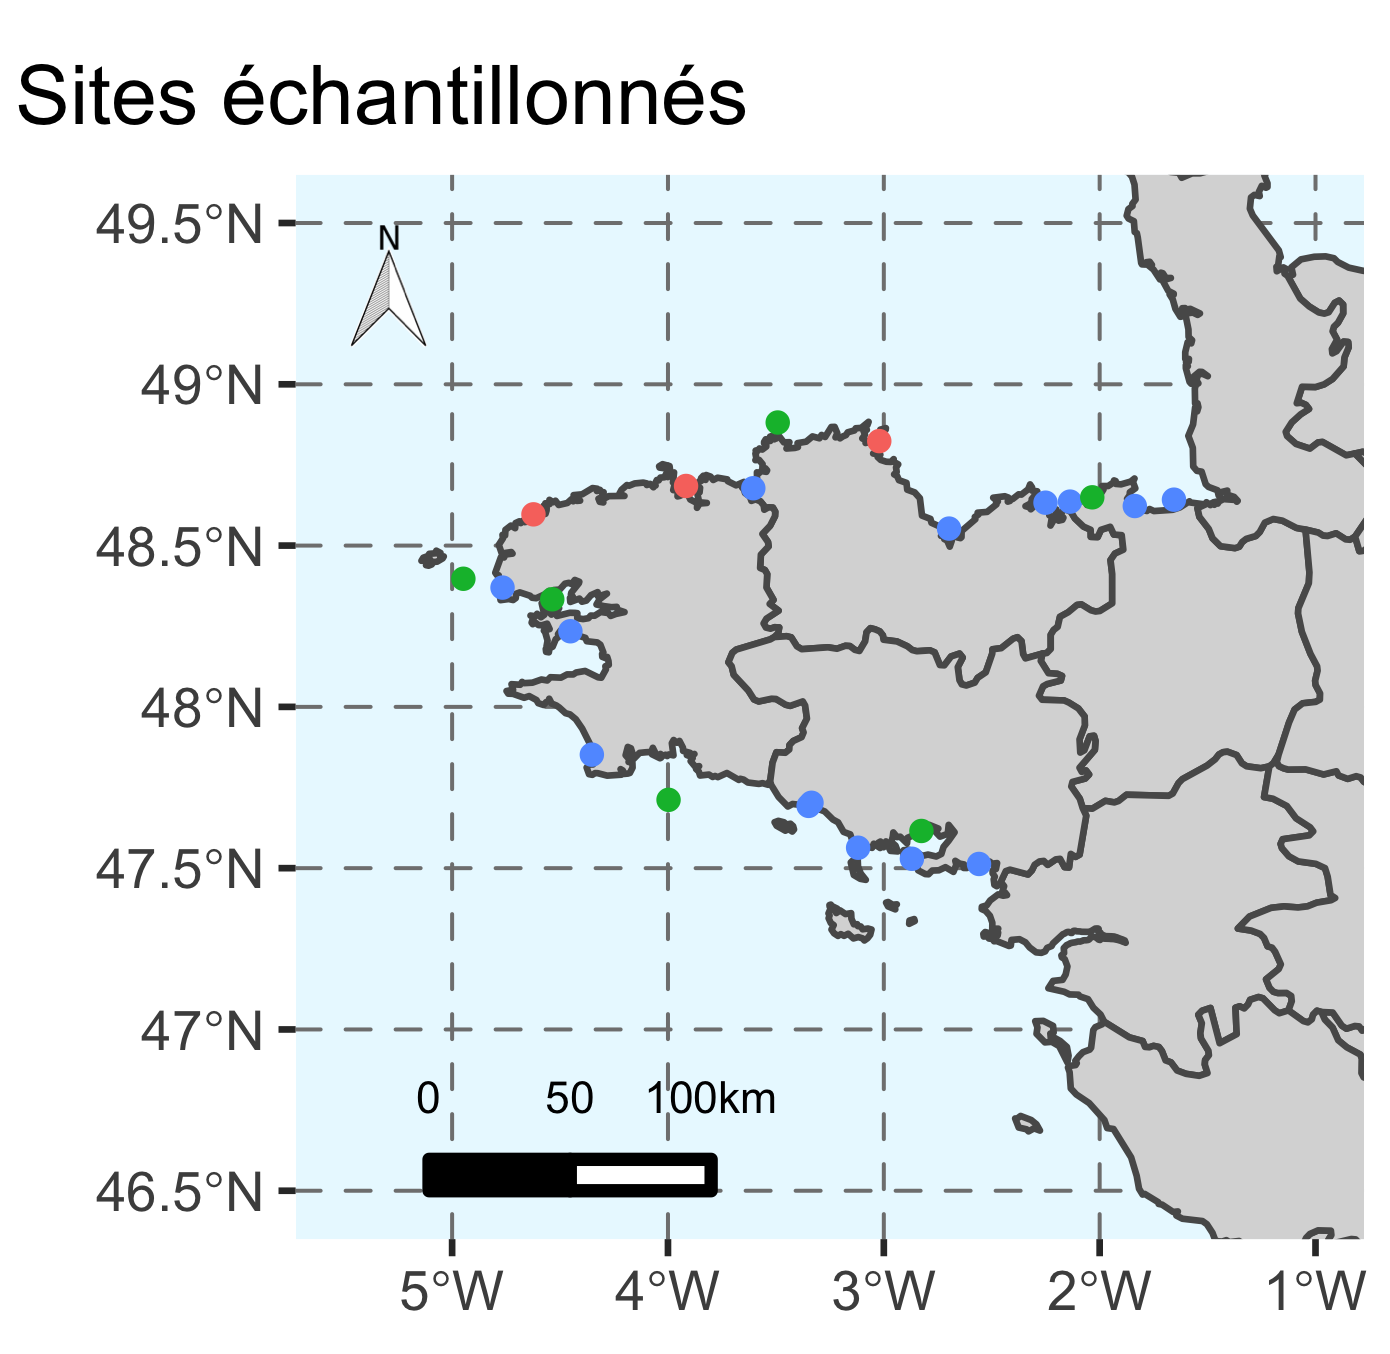
\includegraphics[scale = 0.08]{figs/site_map.png} 
		\end{center}
	\end{figure}
	\end{frame}
 
	\section{Résultats}
	
	\begin{frame}{Performances à l'échelle de l'espèce}
	\begin{figure}[t]
	\begin{center}
		\includegraphics<1>[scale =0.6]{figs/SR2-density-method-2.png}%
		\includegraphics<2>[scale =0.6]{figs/SR2-density-method-3.png}%
		\includegraphics<3>[scale =0.6]{figs/SR2-density-method-4.png}%
	\end{center}
	\end{figure}
	\pause\pause\pause
	Mauvaise capacité de ces modèles à prédire l'abondance des espèces observées :
		\begin{itemize}
			\item \textcolor{green}{Meilleur modèle \emph{HMSC\_hier}} : $24 \leq \text{\emph{RMSE}} \leq 10^4$
			\item \textcolor{red}{Moins bon modèle \emph{GLLVM}} :  $1,25\times10^{31}\leq \text{\emph{RMSE}} \leq 1,09\times 10^{36}$
		\end{itemize}
	\end{frame}
	
	\begin{frame}[c]{Performances à l'échelle de l'espèce}
	\begin{figure}[t]
		\begin{center}
			\includegraphics<1>[scale =0.7]{figs/occurence_1.png}%
			\includegraphics<2>[scale =0.7]{figs/occurence_2.png}%
		\end{center}
	\end{figure}
	\end{frame}
	
	\begin{frame}{Performances à l'échelle de la communauté}
	\begin{figure}[t]
		\captionsetup{justification=centering}
		\caption*{Variations spatio-temporelles de la richesse spécifique}
		\begin{center}
			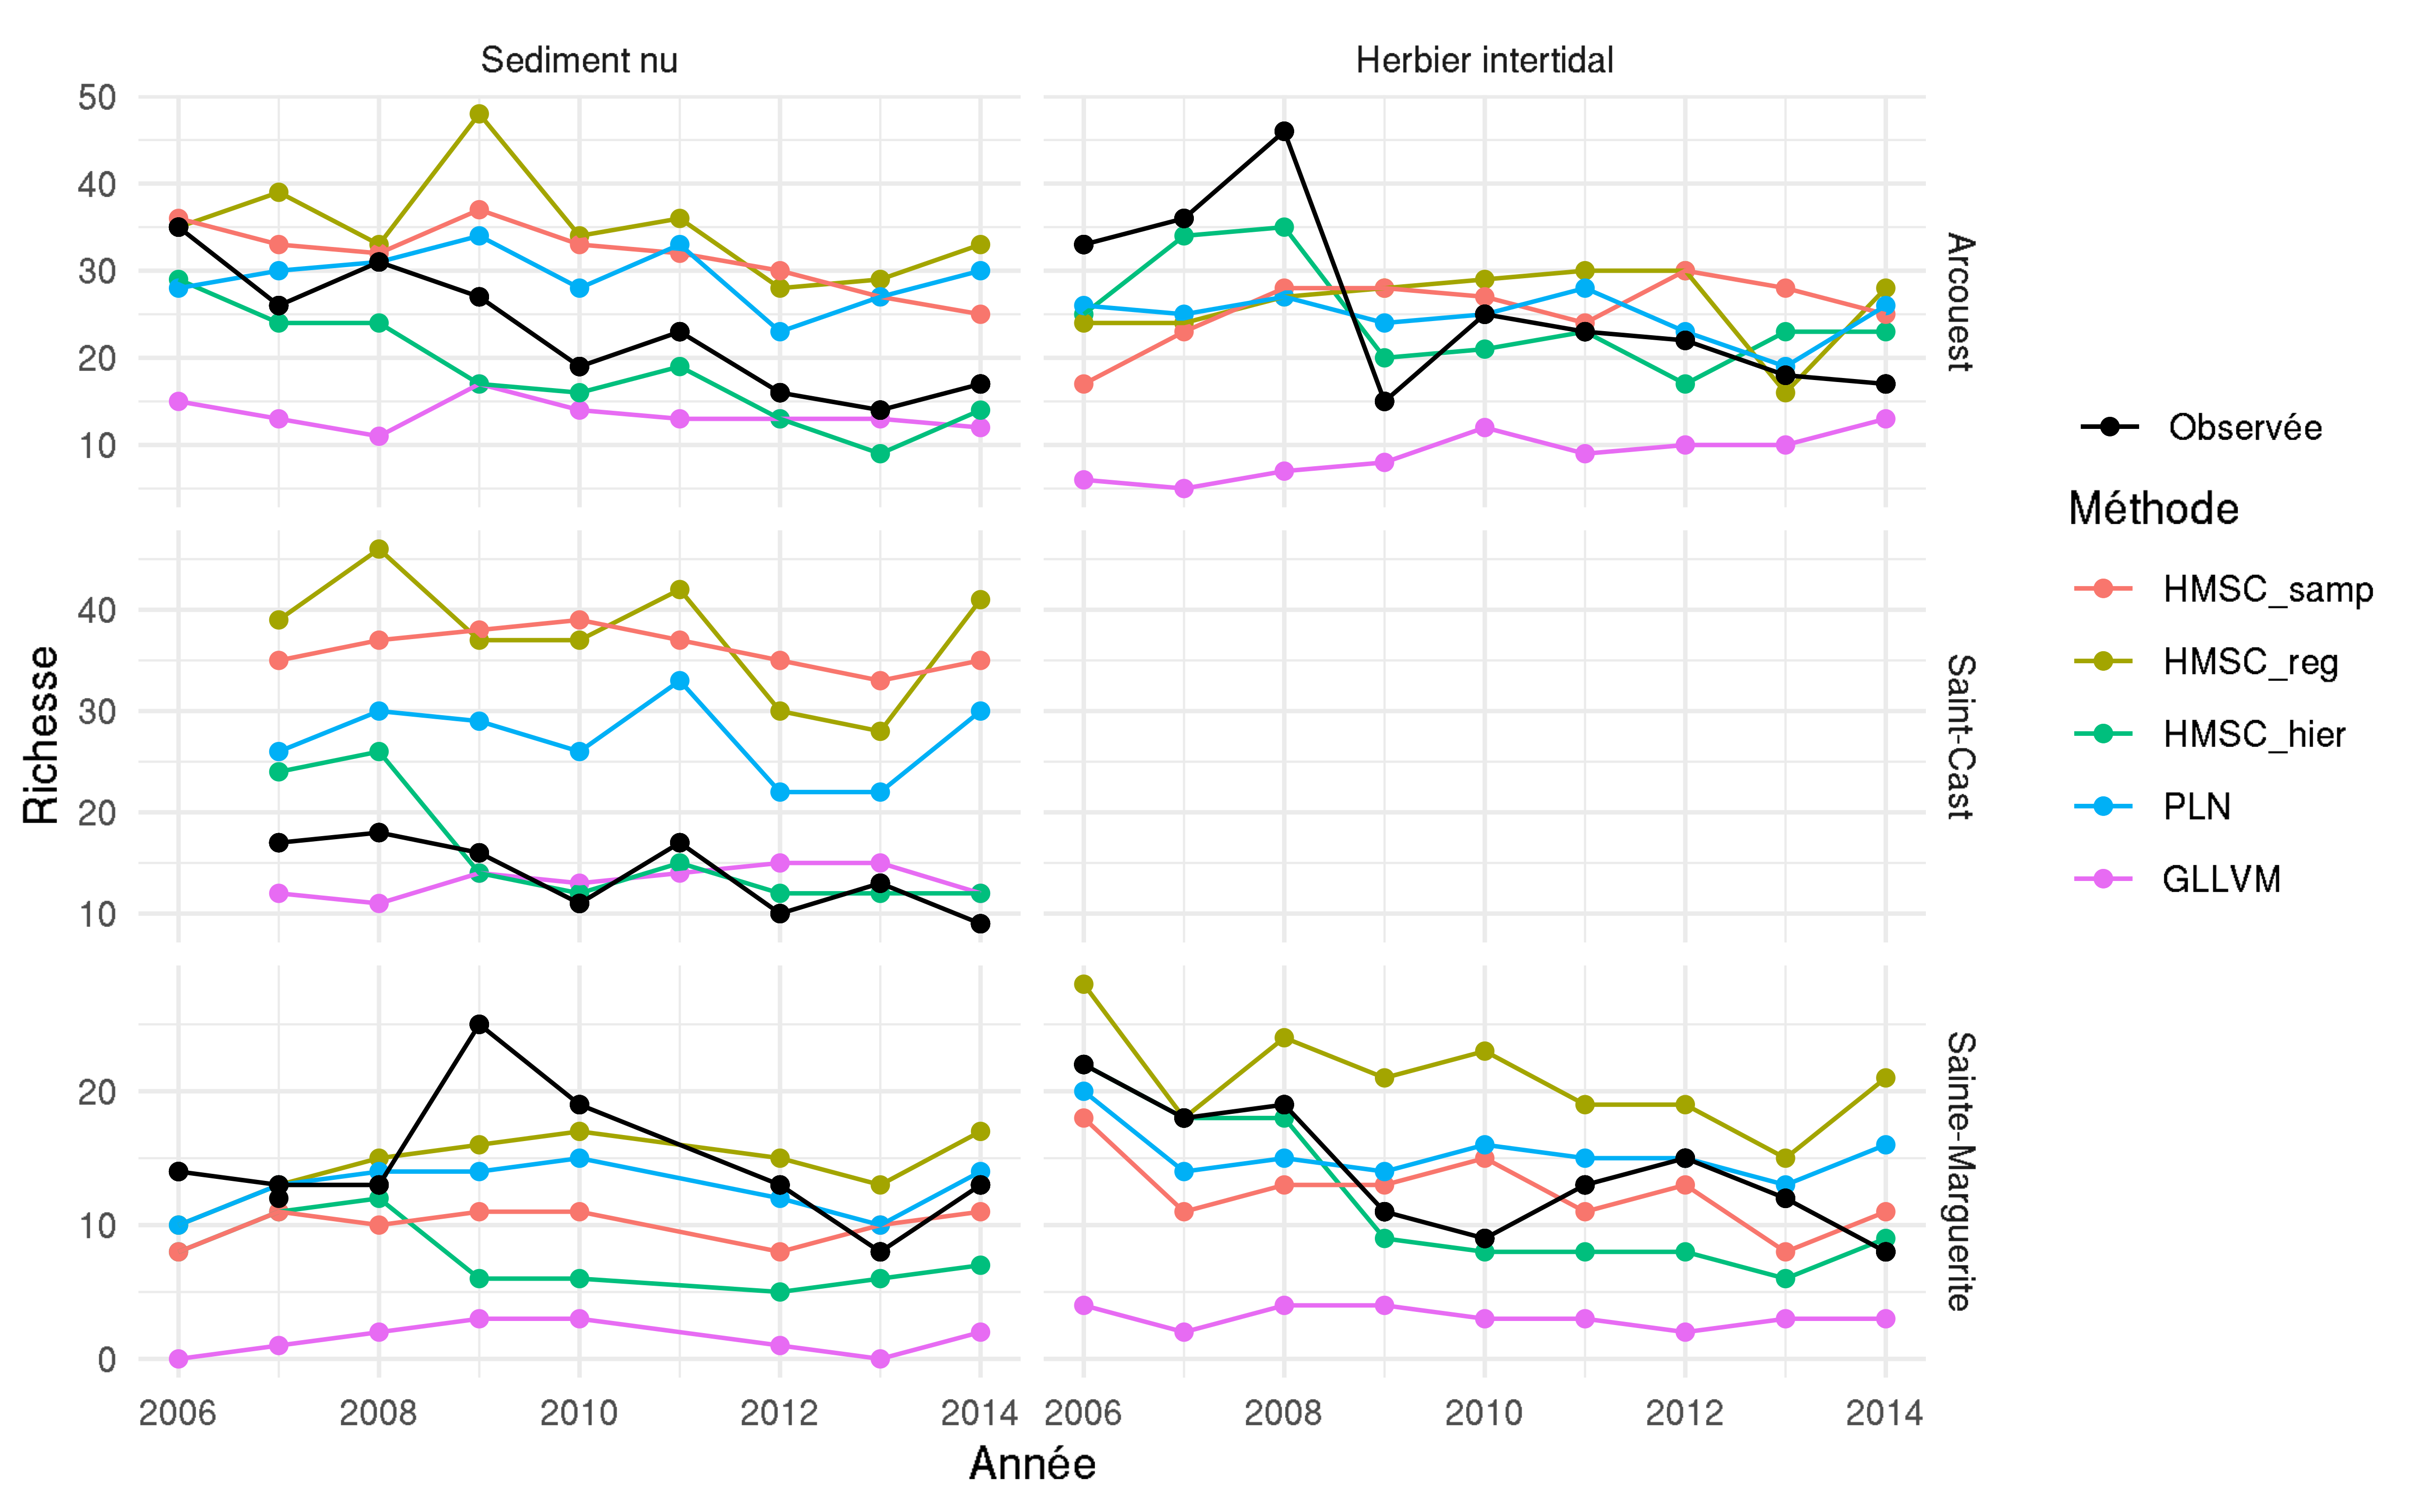
\includegraphics[scale =0.7]{figs/roc-richness-prediction-3.png}
		\end{center}
	\end{figure}
	\end{frame}
	
	\begin{frame}{Performances à l'échelle de la communauté}
	\begin{figure}[t]
		\captionsetup{justification=centering}
		\caption*{Variations spatio-temporelles de la richesse spécifique dans l'herbier de Sainte-Marguerite}
		\begin{center}
			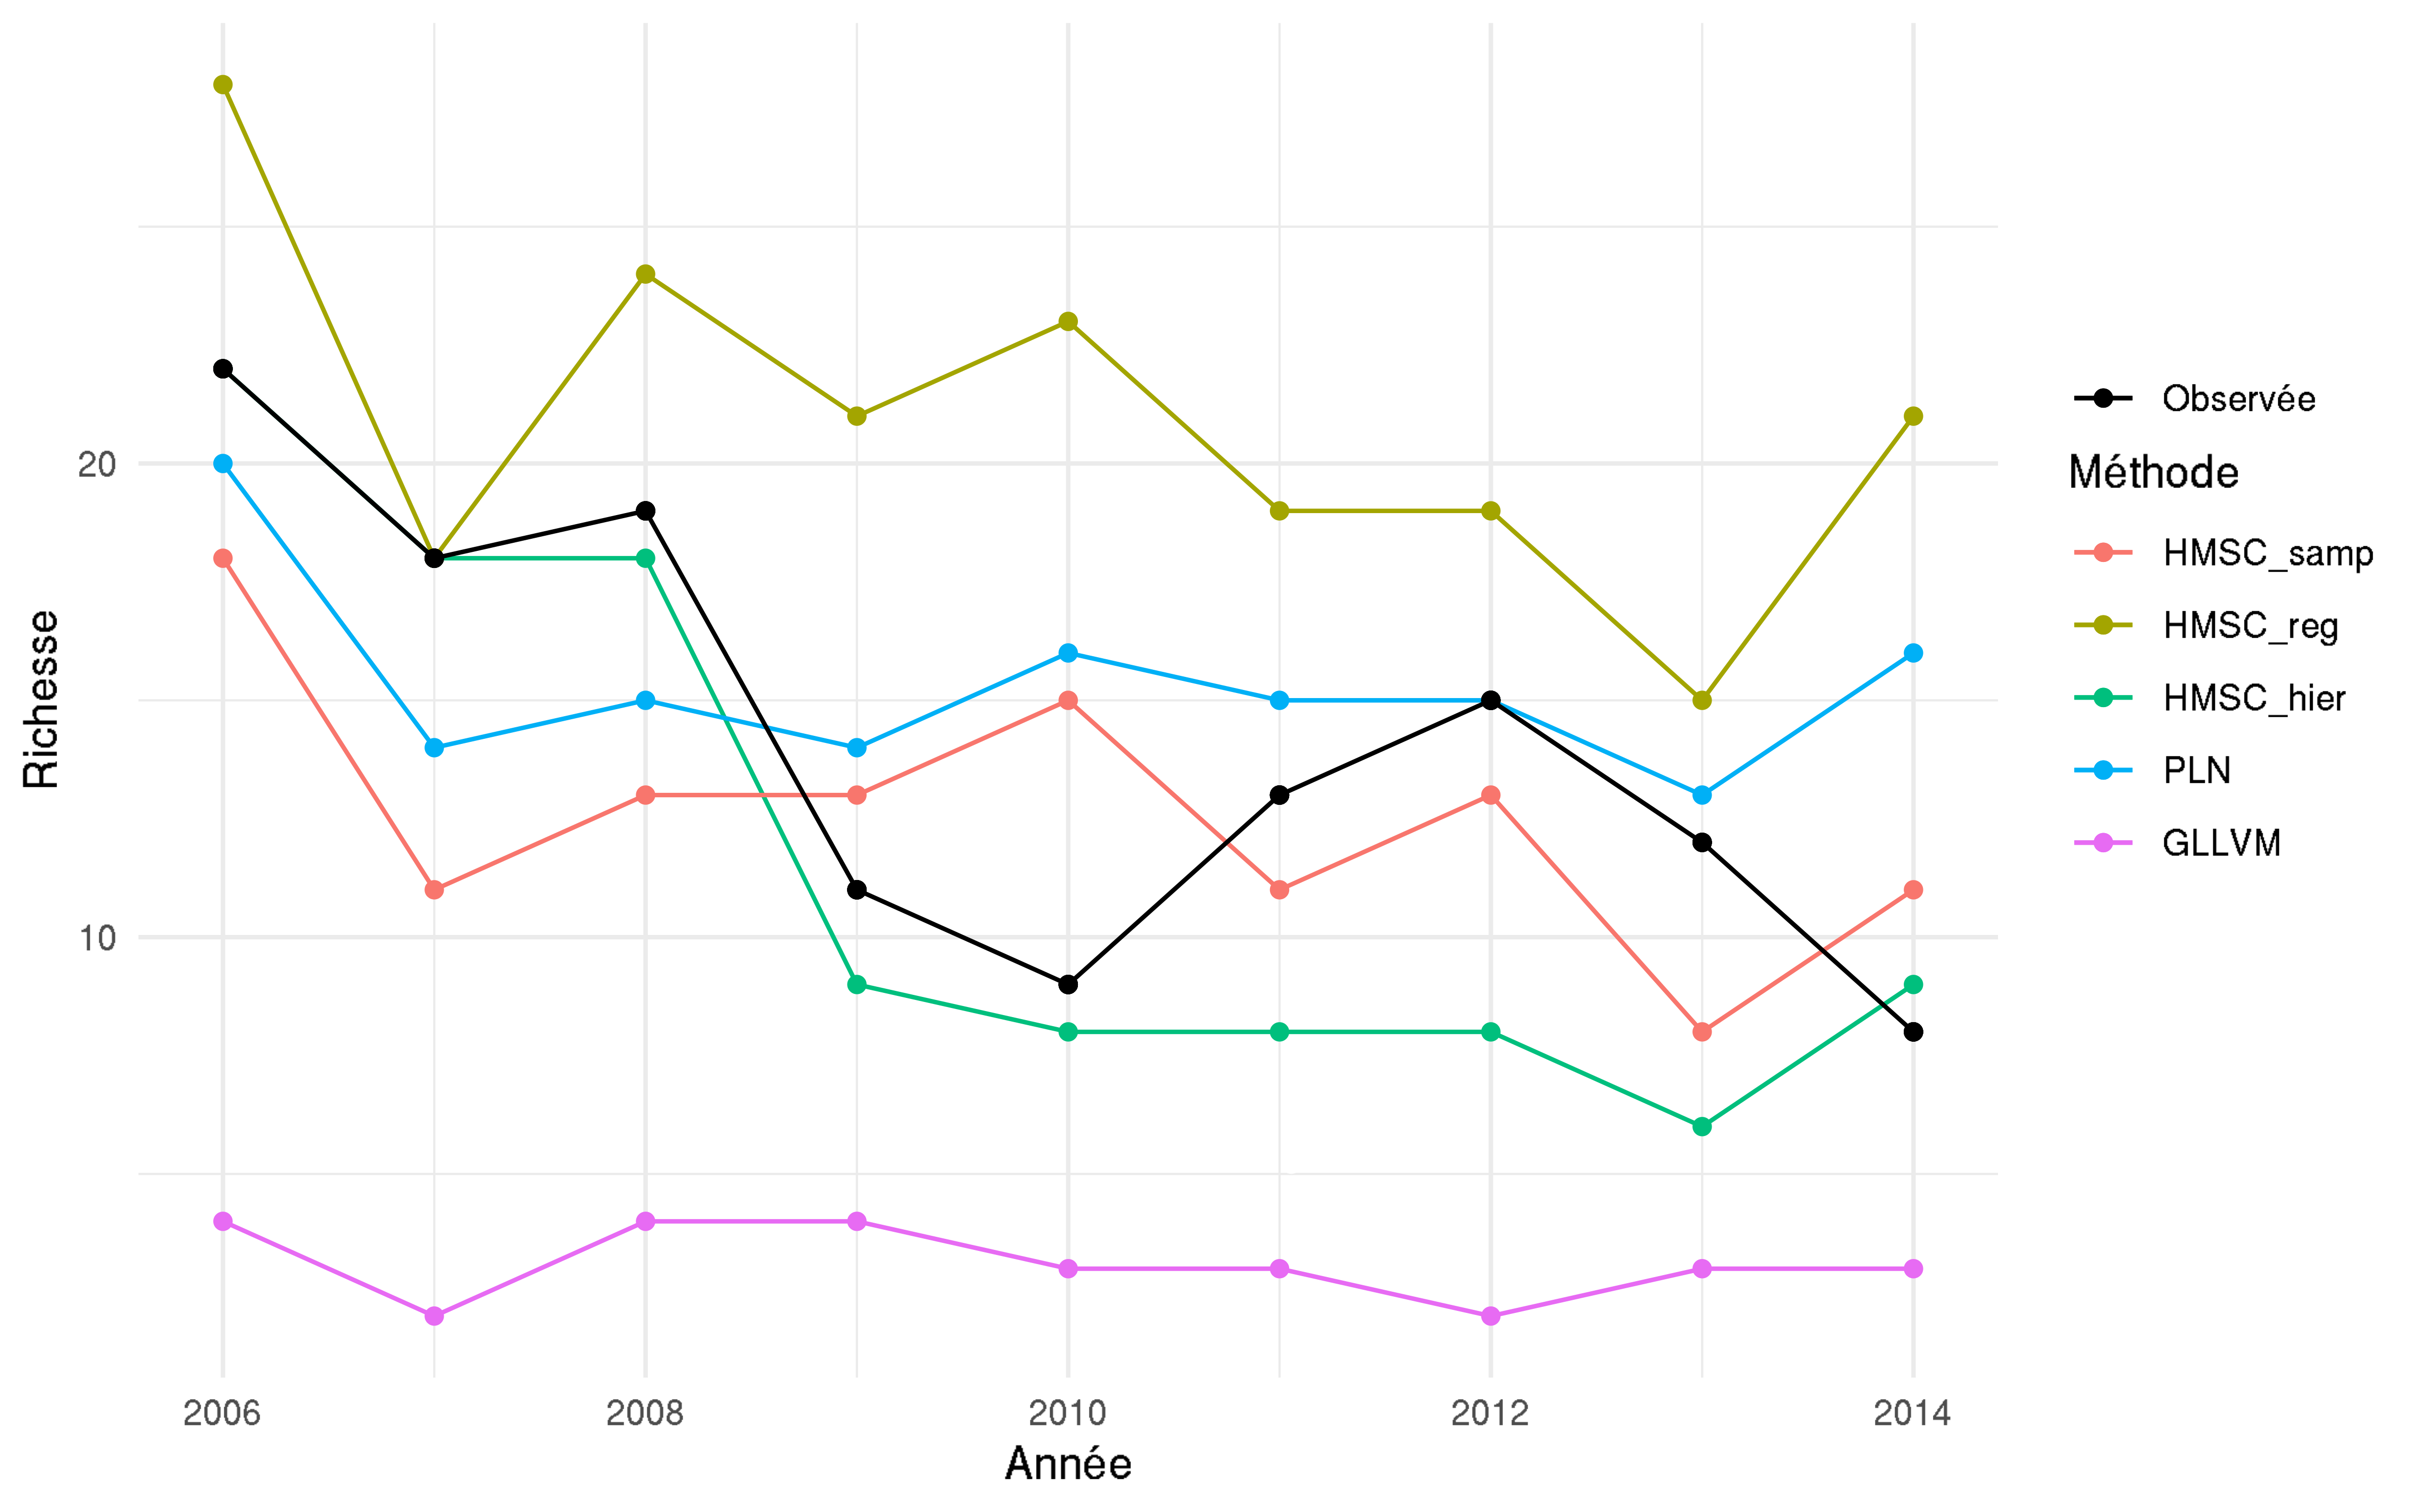
\includegraphics[scale =0.65]{figs/st_marguerite.png}
		\end{center}
	\end{figure}
	\end{frame}
	
	\begin{frame}{Réseau d'interactions reconstruit}
	\begin{figure}[t]
		\begin{center}
			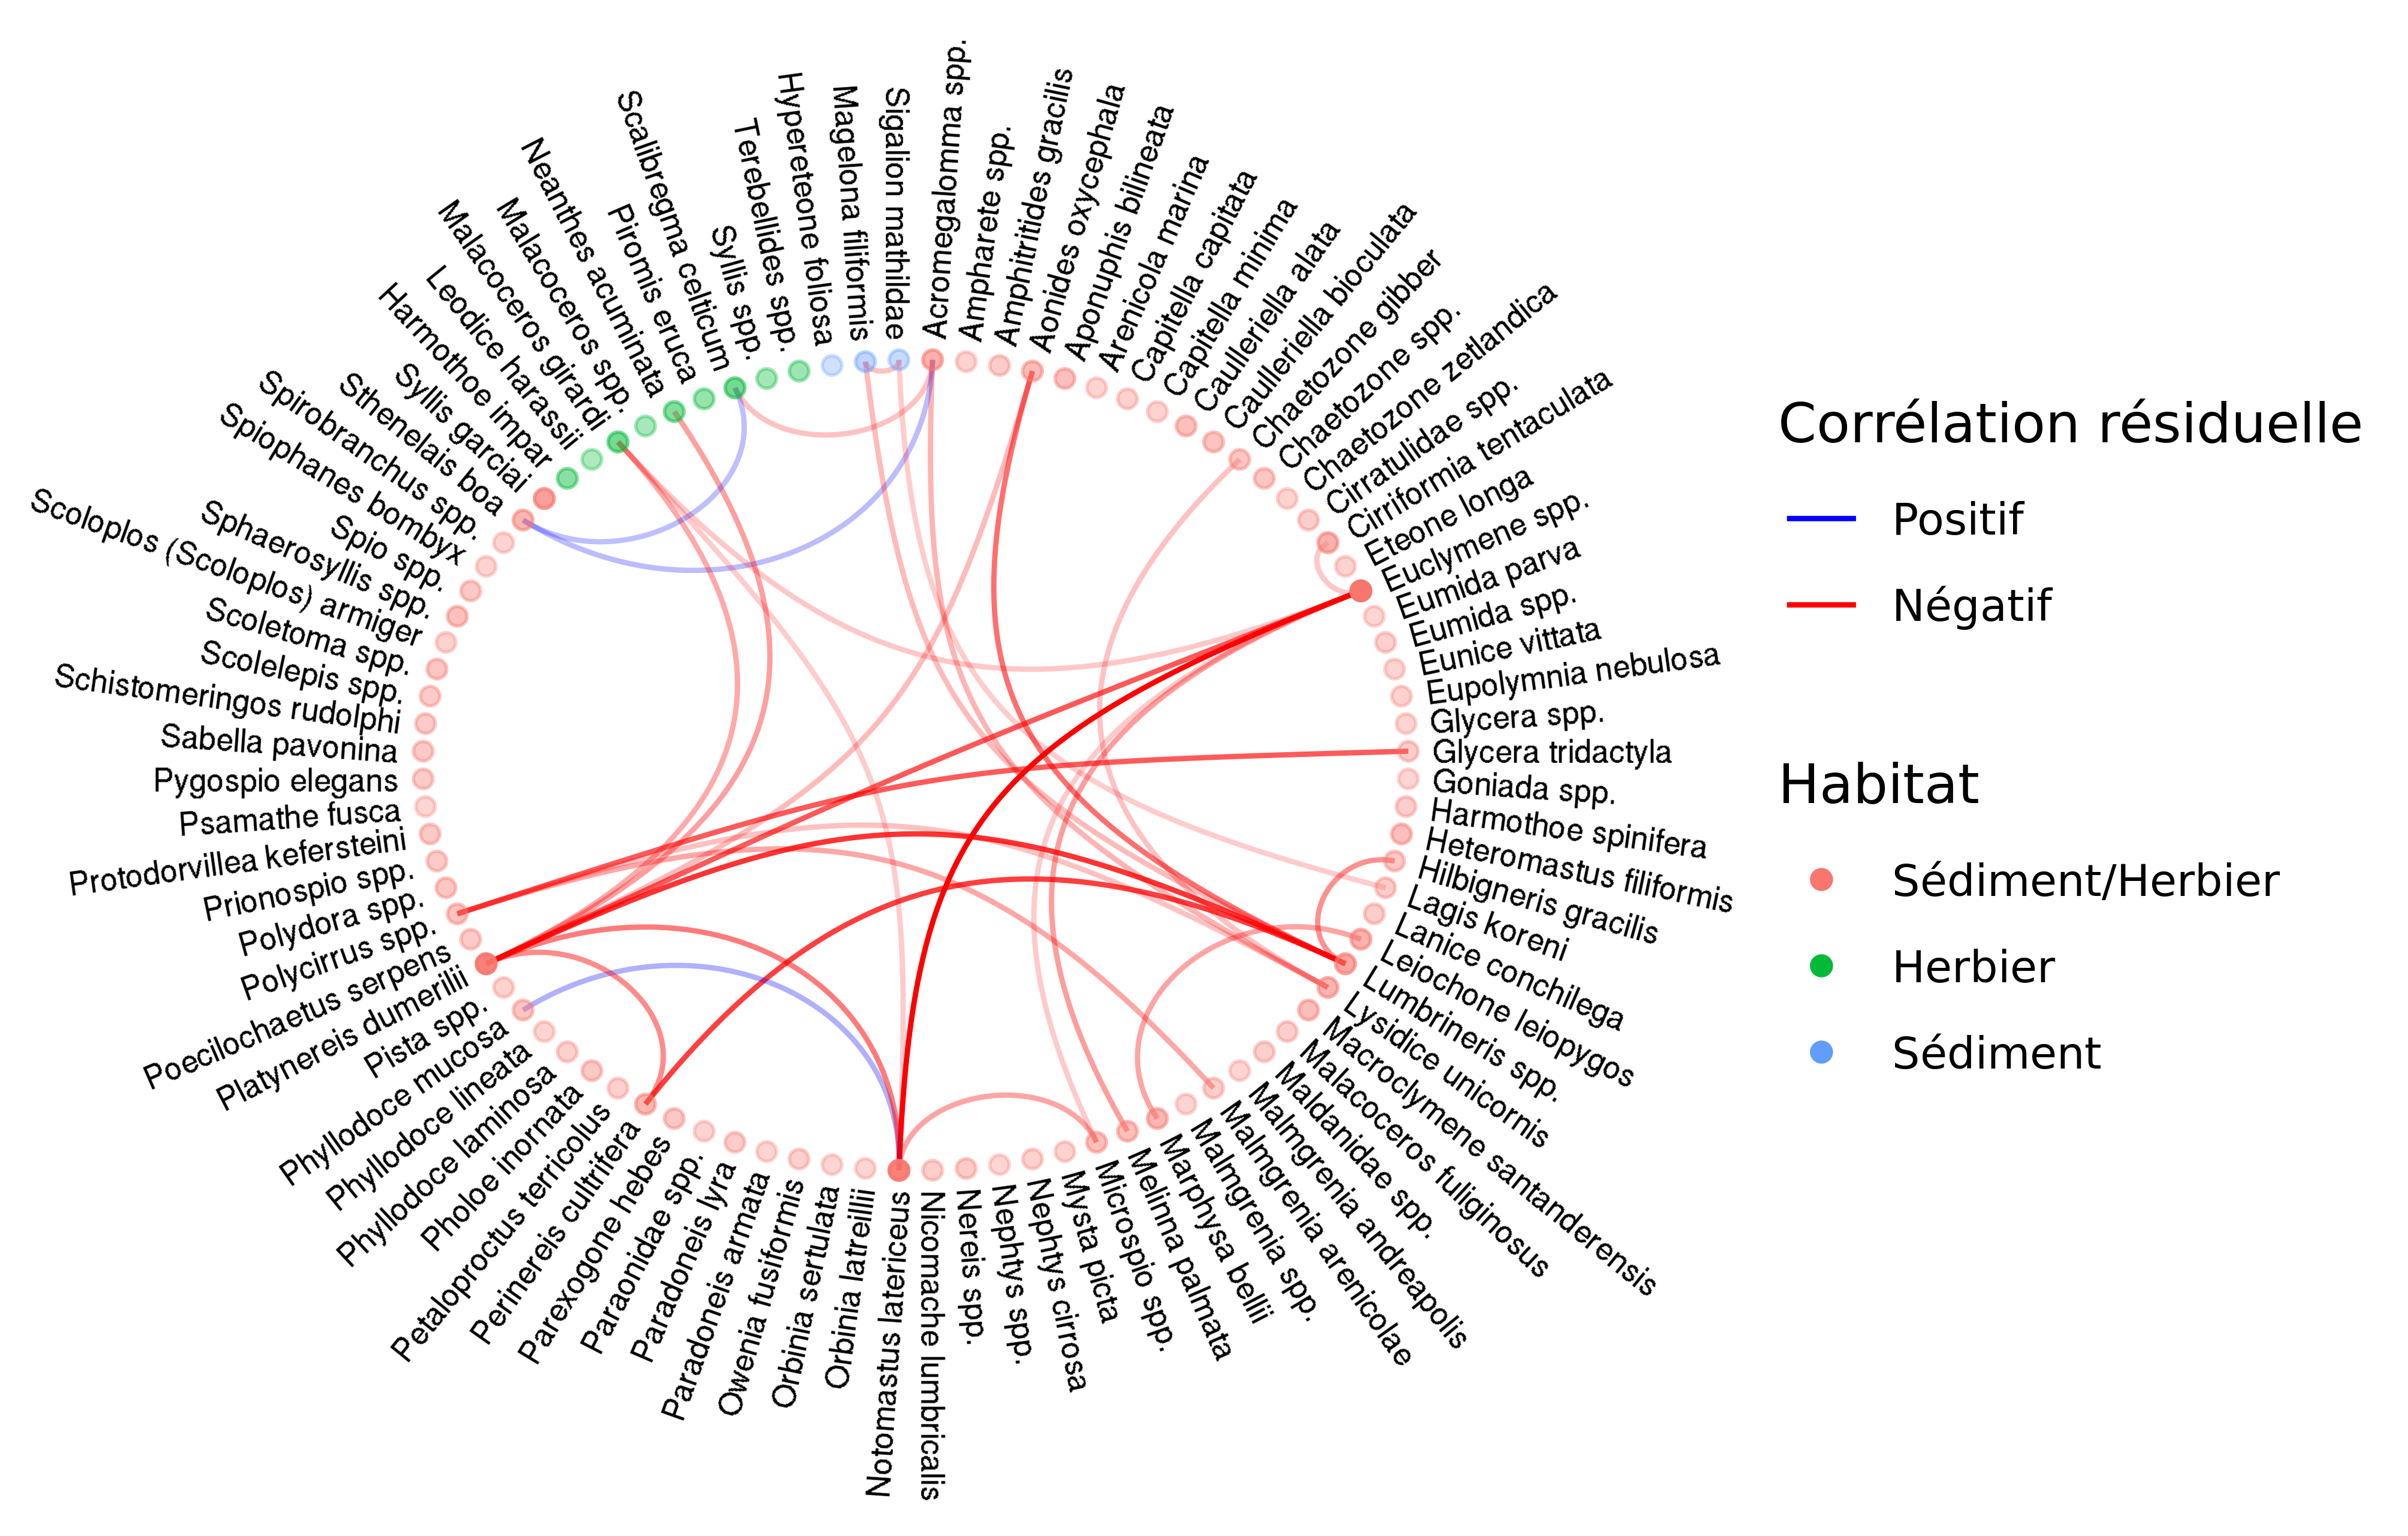
\includegraphics[scale =0.85]{figs/mean-network-1.png}
		\end{center}
	\end{figure}
	\end{frame}
	
	\begin{frame}{Avis experts interactions}
	\begin{figure}[t]
		\begin{center}
			\includegraphics<1>[scale=0.07]{figs/expert-option-1-2.png}
			\includegraphics<2>[scale=0.07]{figs/expert-option-2-2.png}
			\includegraphics<3>[scale=0.07]{figs/expert-option-2-3.png}
		\end{center}
	\end{figure}
	\end{frame}
	
	\section{Discussion \& conclusion}
	\begin{frame}{Discussion}
		\textbf{Mauvaise prédiction de l'abondance} $\rightarrow$ justifie la mise en place de seuil pour prédire l'occurrence\pause\vfill
		\textbf{Bonne prédiction de l'occurrence} $\rightarrow$ variation spatio-temporelle de la richesse spécifique\pause\vfill
		Effets aléatoires $\ggg$ Variables environnementales $\rightarrow$ transférabilité ?\pause\vfill
		\textbf{Difficultés pour inférer des interactions} $\rightarrow$  association entre espèces ?
	\end{frame}
	
	\begin{frame}{Perspectives}
	Améliorer les modèles :\vspace{\baselineskip}\\
	\begin{itemize}
		\item Utiliser des données de traits et/ou phylogénétiques
	\end{itemize}\pause\vspace{4\baselineskip}
	Validation :
	\begin{itemize}
		\item Prédiction de l'abondance \textcolor{red}{\faClose}
		\item Prédiction diversité $\alpha$ \textcolor{green}{\faCheckSquare}
		\item Prédiction diversité $\beta$ \textcolor{blue}{\faQuestionCircle}
	\end{itemize}
	\quad\quad\quad$\rightarrow$ Analyses de trajectoires de communautés~\citep{De_Caceres_2019}
	\end{frame}
	
	\begin{frame}{Perspectives}
	Optimisation numérique indispensable pour des modèles plus compliqués.\vspace{\baselineskip}\\\pause
	\quad\quad\quad$\rightarrow$ Calculs réalisés par DATARMOR.\vfill
		\begin{longtable}[]{lcc}
			\toprule
			Modèle & Temps de calcul & RAM (Go)\tabularnewline
			\midrule
			\endfirsthead
			\toprule
			Modèle & Temps de calcul & RAM (Go)\tabularnewline
			\midrule
			\endhead
			\emph{HMSC\_reg} & 25h 27 min & \(0,49\)\tabularnewline
			\emph{HMSC\_samp} &170h 56 min & \(0,69\)\tabularnewline
			\emph{HMSC\_hier} & \textcolor{red}{457h 50 min} & \(0,73\)\tabularnewline
			\emph{PLN} & \textcolor{green}{3 min} & ~\textcolor{green}{0,37}\tabularnewline
			\emph{GLLVM} & 13h 43 min & \textcolor{red}{68,1}\tabularnewline
			\bottomrule
		\end{longtable}
	
	Choix du modèle : \textbf{trade-off}
	\begin{itemize}
		\item Performances
		\item Coûts de calcul
		\item Flexibilité
	\end{itemize}
	
	\end{frame}
	
	\appendix
	
	\begin{frame}[standout]
		Questions
	\end{frame}
	
	\begin{frame}{Sites échantillonnés}
	\begin{figure}[t]
		\begin{center}
			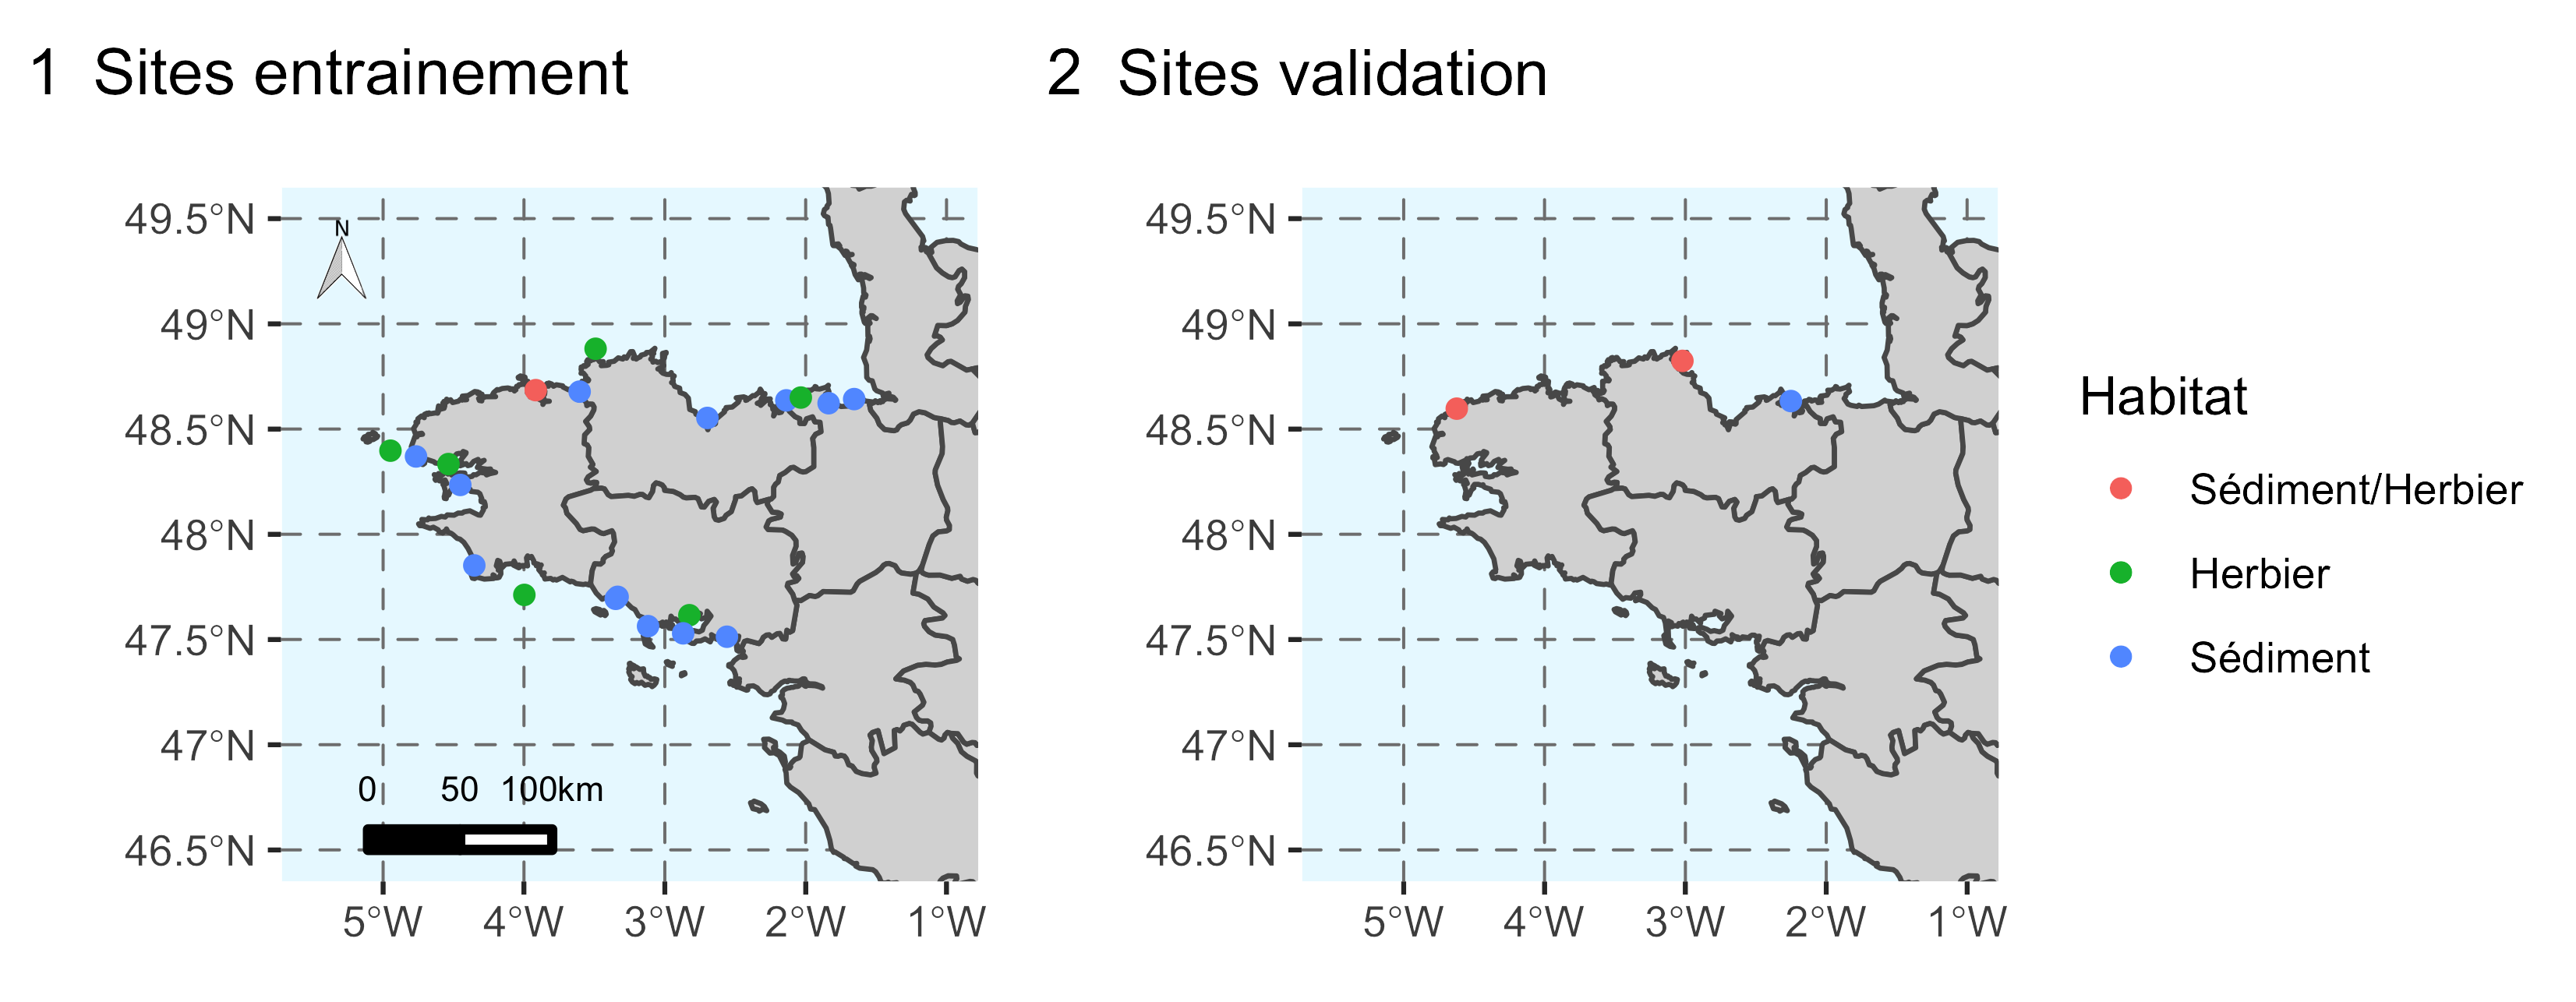
\includegraphics[scale =0.13]{figs/site_map3.png}%
		\end{center}
	\end{figure}
	\end{frame}
	
	\begin{frame}{Effet variables environnementales}
		\begin{figure}[t]
		\begin{center}
			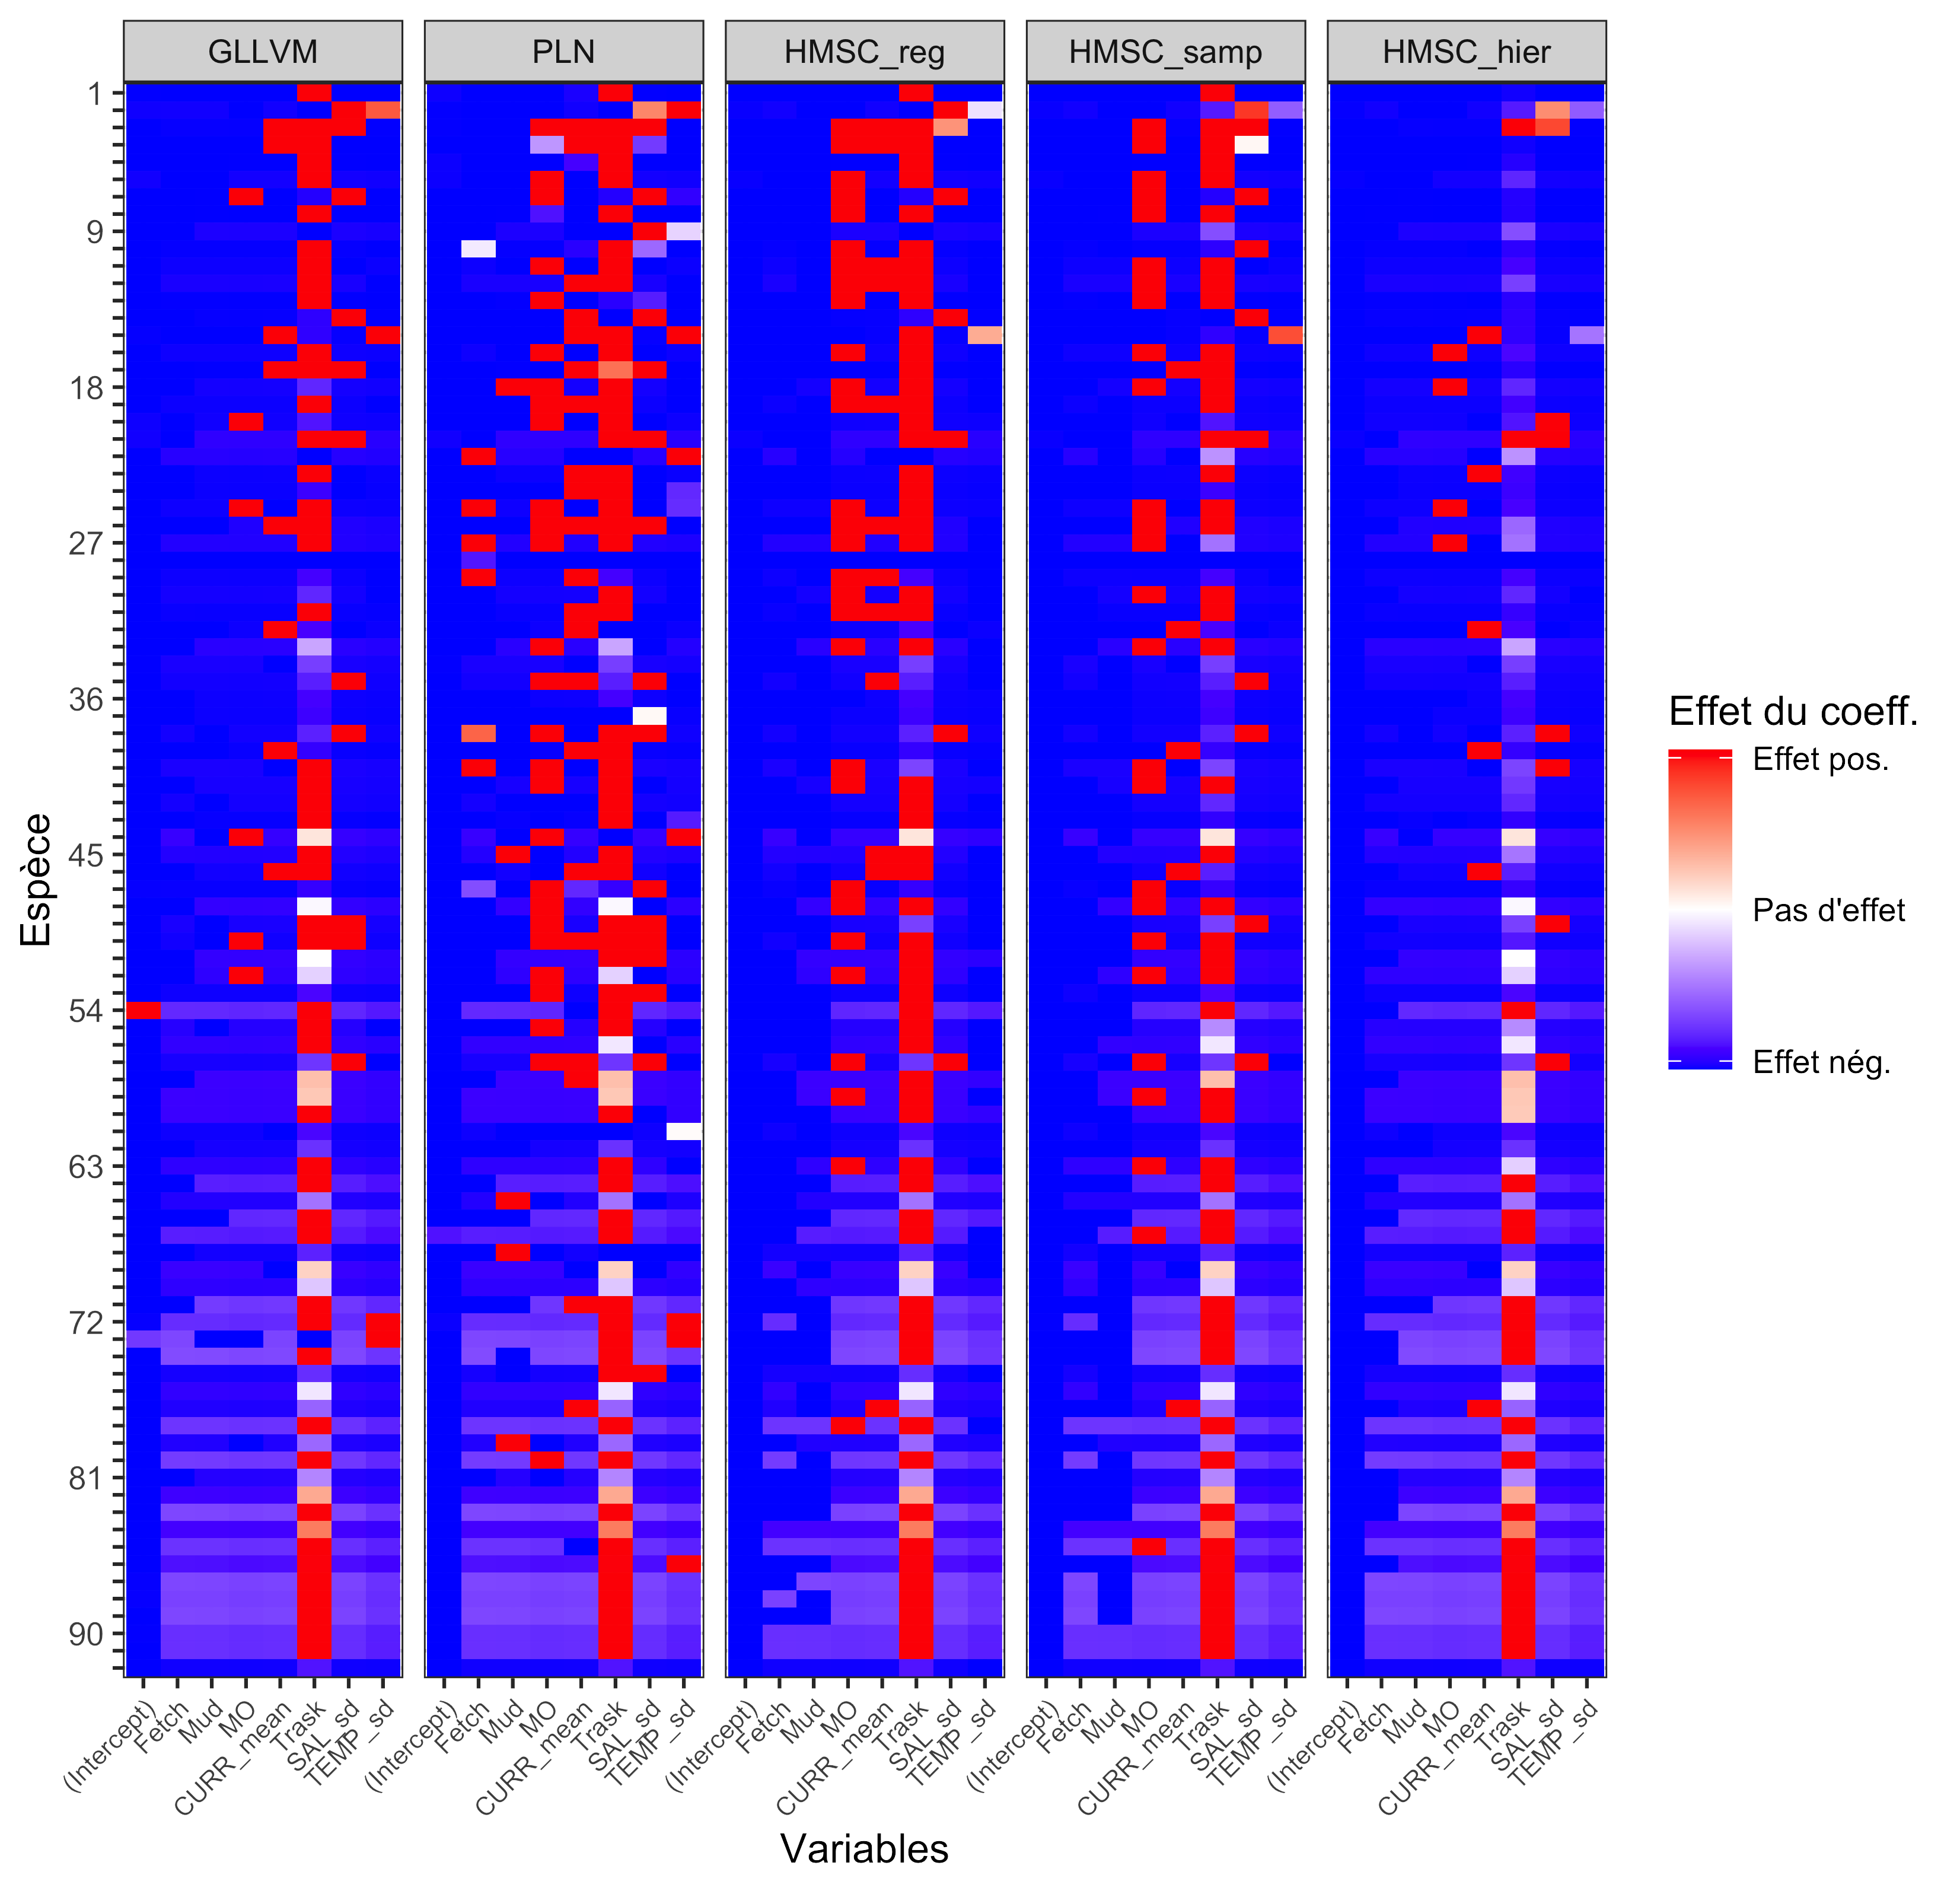
\includegraphics[scale =0.09]{figs/effect_env.png}%
		\end{center}
	\end{figure}
	\end{frame}
	
	\begin{frame}{Partionnement variance expliquée}
		\begin{figure}[t]
		\begin{center}
			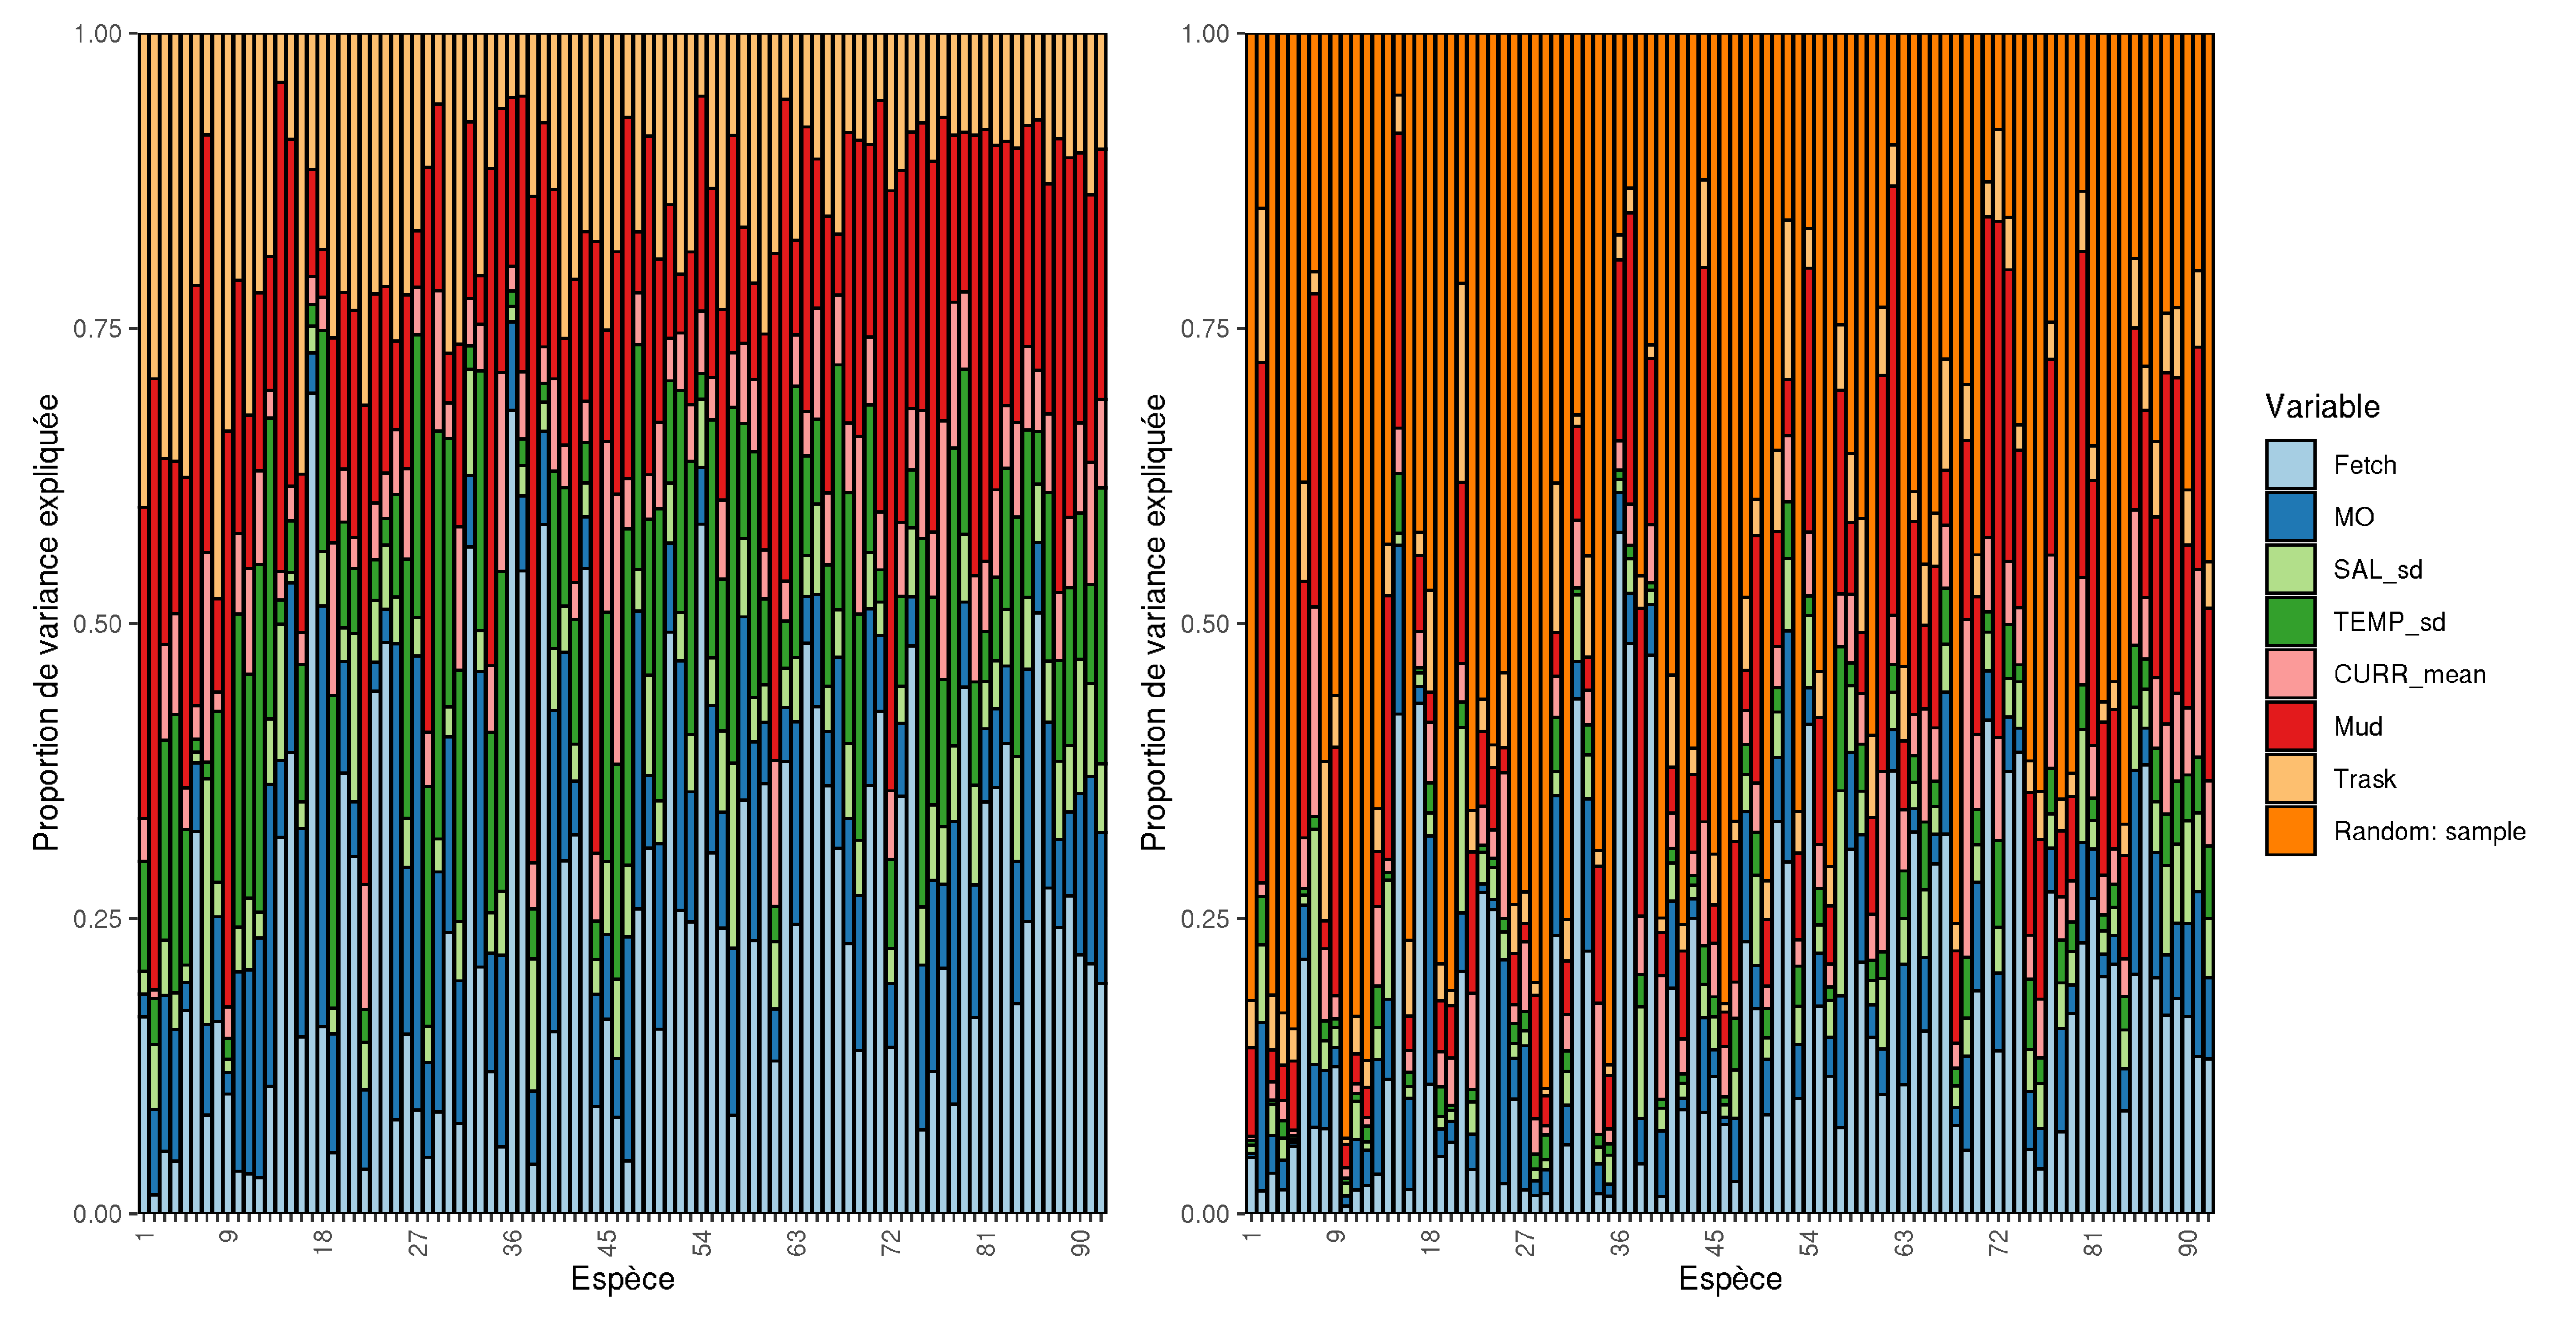
\includegraphics[scale =0.5]{figs/VP_reg_samp.png}%
		\end{center}
	\end{figure}
		$\sigma^2$ variables environnementales : $0,0727\pm 0,061$\\
		$\sigma^2$ effets aléatoires : $0,491\pm 0,239$
	\end{frame}
	
	\begin{frame}{Inférence Réseau}
		\begin{figure}[t]
		\begin{center}
			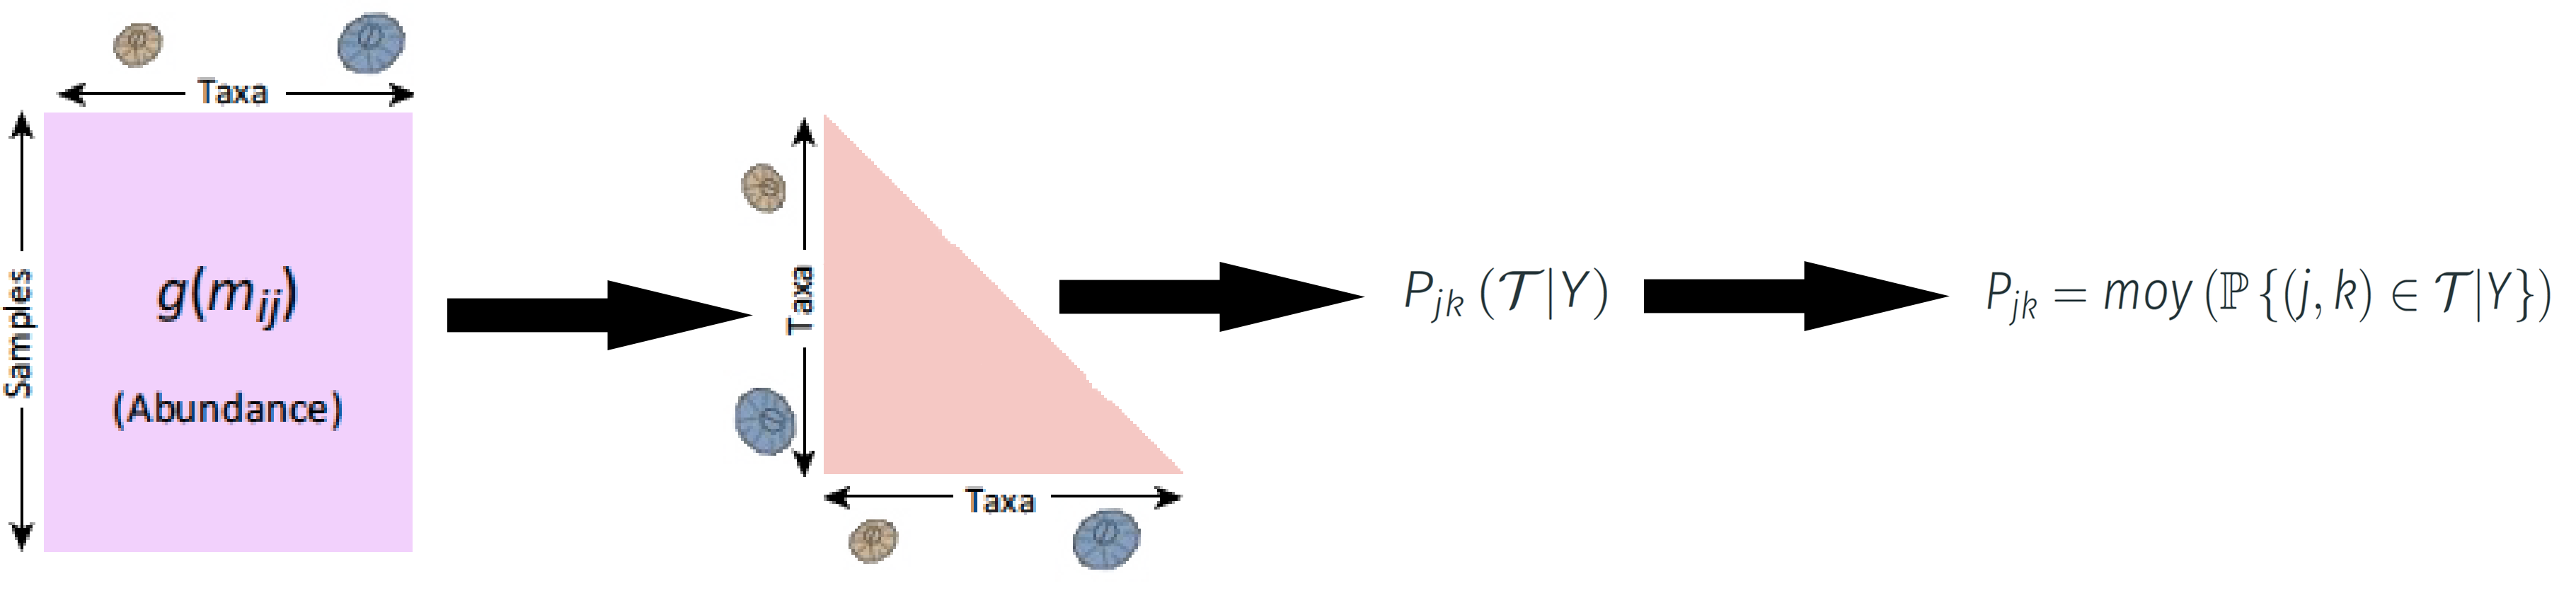
\includegraphics[scale =0.12]{figs/emtree.png}%
		\end{center}
	\end{figure}
	\end{frame}
	
	\begin{frame}[allowframebreaks]{Bibliographie}
			\bibliography{ref_interaction_inference.bib}
	\end{frame}
\end{document}